% Generated by Sphinx.
\def\sphinxdocclass{report}
\documentclass[a4paper,12pt,spanish]{sphinxmanual}
\usepackage[utf8]{inputenc}
\DeclareUnicodeCharacter{00A0}{\nobreakspace}
\usepackage{cmap}
\usepackage[T1]{fontenc}
\usepackage{babel}
\usepackage{times}
\usepackage[Sonny]{fncychap}
\usepackage{longtable}
\usepackage{sphinx}
\usepackage{multirow}

\addto\captionsspanish{\renewcommand{\figurename}{Figura }}
\addto\captionsspanish{\renewcommand{\tablename}{Tabla }}
\floatname{literal-block}{Lista }


  \setcounter{tocdepth}{2}
  \fancypagestyle{normal}{
    \fancyhf{}
    % Footer

    \fancyfoot[LE,RO]{{\textbf{\textsf{\thepage}}}}
    \fancyfoot[LO]{{\sffamily\bfseries\nouppercase{\textbf{\rightmark}}}}
    \fancyfoot[RE]{{\sffamily\bfseries\nouppercase{\textbf{\leftmark}}}}

    \fancyhead[LE,RO]{{\sffamily\bfseries\nouppercase{\textit{Introducción al desarrollo de software}}}}

    \renewcommand{\headrulewidth}{0.4pt}
    \renewcommand{\footrulewidth}{0.4pt}
  }
  % Update the plain style so we get the page number & footer line,
  % but not a chapter or section title.  This is to keep the first
  % page of a chapter and the blank page between chapters `clean.'
  \fancypagestyle{plain}{
    \fancyhf{}
    \fancyfoot[RO,RE]{{\textbf{\textsf{\thepage}}}}
    \renewcommand{\headrulewidth}{0pt}
    \renewcommand{\footrulewidth}{0.4pt}
  }


\title{Introducción al desarrollo de software}
\date{14 de August de 2015}
\release{1.0}
\author{Emiliano López}
\newcommand{\sphinxlogo}{}
\renewcommand{\releasename}{Publicación}
\makeindex

\makeatletter
\def\PYG@reset{\let\PYG@it=\relax \let\PYG@bf=\relax%
    \let\PYG@ul=\relax \let\PYG@tc=\relax%
    \let\PYG@bc=\relax \let\PYG@ff=\relax}
\def\PYG@tok#1{\csname PYG@tok@#1\endcsname}
\def\PYG@toks#1+{\ifx\relax#1\empty\else%
    \PYG@tok{#1}\expandafter\PYG@toks\fi}
\def\PYG@do#1{\PYG@bc{\PYG@tc{\PYG@ul{%
    \PYG@it{\PYG@bf{\PYG@ff{#1}}}}}}}
\def\PYG#1#2{\PYG@reset\PYG@toks#1+\relax+\PYG@do{#2}}

\expandafter\def\csname PYG@tok@gd\endcsname{\def\PYG@tc##1{\textcolor[rgb]{0.63,0.00,0.00}{##1}}}
\expandafter\def\csname PYG@tok@gu\endcsname{\let\PYG@bf=\textbf\def\PYG@tc##1{\textcolor[rgb]{0.50,0.00,0.50}{##1}}}
\expandafter\def\csname PYG@tok@gt\endcsname{\def\PYG@tc##1{\textcolor[rgb]{0.00,0.27,0.87}{##1}}}
\expandafter\def\csname PYG@tok@gs\endcsname{\let\PYG@bf=\textbf}
\expandafter\def\csname PYG@tok@gr\endcsname{\def\PYG@tc##1{\textcolor[rgb]{1.00,0.00,0.00}{##1}}}
\expandafter\def\csname PYG@tok@cm\endcsname{\let\PYG@it=\textit\def\PYG@tc##1{\textcolor[rgb]{0.25,0.50,0.56}{##1}}}
\expandafter\def\csname PYG@tok@vg\endcsname{\def\PYG@tc##1{\textcolor[rgb]{0.73,0.38,0.84}{##1}}}
\expandafter\def\csname PYG@tok@m\endcsname{\def\PYG@tc##1{\textcolor[rgb]{0.13,0.50,0.31}{##1}}}
\expandafter\def\csname PYG@tok@mh\endcsname{\def\PYG@tc##1{\textcolor[rgb]{0.13,0.50,0.31}{##1}}}
\expandafter\def\csname PYG@tok@cs\endcsname{\def\PYG@tc##1{\textcolor[rgb]{0.25,0.50,0.56}{##1}}\def\PYG@bc##1{\setlength{\fboxsep}{0pt}\colorbox[rgb]{1.00,0.94,0.94}{\strut ##1}}}
\expandafter\def\csname PYG@tok@ge\endcsname{\let\PYG@it=\textit}
\expandafter\def\csname PYG@tok@vc\endcsname{\def\PYG@tc##1{\textcolor[rgb]{0.73,0.38,0.84}{##1}}}
\expandafter\def\csname PYG@tok@il\endcsname{\def\PYG@tc##1{\textcolor[rgb]{0.13,0.50,0.31}{##1}}}
\expandafter\def\csname PYG@tok@go\endcsname{\def\PYG@tc##1{\textcolor[rgb]{0.20,0.20,0.20}{##1}}}
\expandafter\def\csname PYG@tok@cp\endcsname{\def\PYG@tc##1{\textcolor[rgb]{0.00,0.44,0.13}{##1}}}
\expandafter\def\csname PYG@tok@gi\endcsname{\def\PYG@tc##1{\textcolor[rgb]{0.00,0.63,0.00}{##1}}}
\expandafter\def\csname PYG@tok@gh\endcsname{\let\PYG@bf=\textbf\def\PYG@tc##1{\textcolor[rgb]{0.00,0.00,0.50}{##1}}}
\expandafter\def\csname PYG@tok@ni\endcsname{\let\PYG@bf=\textbf\def\PYG@tc##1{\textcolor[rgb]{0.84,0.33,0.22}{##1}}}
\expandafter\def\csname PYG@tok@nl\endcsname{\let\PYG@bf=\textbf\def\PYG@tc##1{\textcolor[rgb]{0.00,0.13,0.44}{##1}}}
\expandafter\def\csname PYG@tok@nn\endcsname{\let\PYG@bf=\textbf\def\PYG@tc##1{\textcolor[rgb]{0.05,0.52,0.71}{##1}}}
\expandafter\def\csname PYG@tok@no\endcsname{\def\PYG@tc##1{\textcolor[rgb]{0.38,0.68,0.84}{##1}}}
\expandafter\def\csname PYG@tok@na\endcsname{\def\PYG@tc##1{\textcolor[rgb]{0.25,0.44,0.63}{##1}}}
\expandafter\def\csname PYG@tok@nb\endcsname{\def\PYG@tc##1{\textcolor[rgb]{0.00,0.44,0.13}{##1}}}
\expandafter\def\csname PYG@tok@nc\endcsname{\let\PYG@bf=\textbf\def\PYG@tc##1{\textcolor[rgb]{0.05,0.52,0.71}{##1}}}
\expandafter\def\csname PYG@tok@nd\endcsname{\let\PYG@bf=\textbf\def\PYG@tc##1{\textcolor[rgb]{0.33,0.33,0.33}{##1}}}
\expandafter\def\csname PYG@tok@ne\endcsname{\def\PYG@tc##1{\textcolor[rgb]{0.00,0.44,0.13}{##1}}}
\expandafter\def\csname PYG@tok@nf\endcsname{\def\PYG@tc##1{\textcolor[rgb]{0.02,0.16,0.49}{##1}}}
\expandafter\def\csname PYG@tok@si\endcsname{\let\PYG@it=\textit\def\PYG@tc##1{\textcolor[rgb]{0.44,0.63,0.82}{##1}}}
\expandafter\def\csname PYG@tok@s2\endcsname{\def\PYG@tc##1{\textcolor[rgb]{0.25,0.44,0.63}{##1}}}
\expandafter\def\csname PYG@tok@vi\endcsname{\def\PYG@tc##1{\textcolor[rgb]{0.73,0.38,0.84}{##1}}}
\expandafter\def\csname PYG@tok@nt\endcsname{\let\PYG@bf=\textbf\def\PYG@tc##1{\textcolor[rgb]{0.02,0.16,0.45}{##1}}}
\expandafter\def\csname PYG@tok@nv\endcsname{\def\PYG@tc##1{\textcolor[rgb]{0.73,0.38,0.84}{##1}}}
\expandafter\def\csname PYG@tok@s1\endcsname{\def\PYG@tc##1{\textcolor[rgb]{0.25,0.44,0.63}{##1}}}
\expandafter\def\csname PYG@tok@gp\endcsname{\let\PYG@bf=\textbf\def\PYG@tc##1{\textcolor[rgb]{0.78,0.36,0.04}{##1}}}
\expandafter\def\csname PYG@tok@sh\endcsname{\def\PYG@tc##1{\textcolor[rgb]{0.25,0.44,0.63}{##1}}}
\expandafter\def\csname PYG@tok@ow\endcsname{\let\PYG@bf=\textbf\def\PYG@tc##1{\textcolor[rgb]{0.00,0.44,0.13}{##1}}}
\expandafter\def\csname PYG@tok@sx\endcsname{\def\PYG@tc##1{\textcolor[rgb]{0.78,0.36,0.04}{##1}}}
\expandafter\def\csname PYG@tok@bp\endcsname{\def\PYG@tc##1{\textcolor[rgb]{0.00,0.44,0.13}{##1}}}
\expandafter\def\csname PYG@tok@c1\endcsname{\let\PYG@it=\textit\def\PYG@tc##1{\textcolor[rgb]{0.25,0.50,0.56}{##1}}}
\expandafter\def\csname PYG@tok@kc\endcsname{\let\PYG@bf=\textbf\def\PYG@tc##1{\textcolor[rgb]{0.00,0.44,0.13}{##1}}}
\expandafter\def\csname PYG@tok@c\endcsname{\let\PYG@it=\textit\def\PYG@tc##1{\textcolor[rgb]{0.25,0.50,0.56}{##1}}}
\expandafter\def\csname PYG@tok@mf\endcsname{\def\PYG@tc##1{\textcolor[rgb]{0.13,0.50,0.31}{##1}}}
\expandafter\def\csname PYG@tok@err\endcsname{\def\PYG@bc##1{\setlength{\fboxsep}{0pt}\fcolorbox[rgb]{1.00,0.00,0.00}{1,1,1}{\strut ##1}}}
\expandafter\def\csname PYG@tok@mb\endcsname{\def\PYG@tc##1{\textcolor[rgb]{0.13,0.50,0.31}{##1}}}
\expandafter\def\csname PYG@tok@ss\endcsname{\def\PYG@tc##1{\textcolor[rgb]{0.32,0.47,0.09}{##1}}}
\expandafter\def\csname PYG@tok@sr\endcsname{\def\PYG@tc##1{\textcolor[rgb]{0.14,0.33,0.53}{##1}}}
\expandafter\def\csname PYG@tok@mo\endcsname{\def\PYG@tc##1{\textcolor[rgb]{0.13,0.50,0.31}{##1}}}
\expandafter\def\csname PYG@tok@kd\endcsname{\let\PYG@bf=\textbf\def\PYG@tc##1{\textcolor[rgb]{0.00,0.44,0.13}{##1}}}
\expandafter\def\csname PYG@tok@mi\endcsname{\def\PYG@tc##1{\textcolor[rgb]{0.13,0.50,0.31}{##1}}}
\expandafter\def\csname PYG@tok@kn\endcsname{\let\PYG@bf=\textbf\def\PYG@tc##1{\textcolor[rgb]{0.00,0.44,0.13}{##1}}}
\expandafter\def\csname PYG@tok@o\endcsname{\def\PYG@tc##1{\textcolor[rgb]{0.40,0.40,0.40}{##1}}}
\expandafter\def\csname PYG@tok@kr\endcsname{\let\PYG@bf=\textbf\def\PYG@tc##1{\textcolor[rgb]{0.00,0.44,0.13}{##1}}}
\expandafter\def\csname PYG@tok@s\endcsname{\def\PYG@tc##1{\textcolor[rgb]{0.25,0.44,0.63}{##1}}}
\expandafter\def\csname PYG@tok@kp\endcsname{\def\PYG@tc##1{\textcolor[rgb]{0.00,0.44,0.13}{##1}}}
\expandafter\def\csname PYG@tok@w\endcsname{\def\PYG@tc##1{\textcolor[rgb]{0.73,0.73,0.73}{##1}}}
\expandafter\def\csname PYG@tok@kt\endcsname{\def\PYG@tc##1{\textcolor[rgb]{0.56,0.13,0.00}{##1}}}
\expandafter\def\csname PYG@tok@sc\endcsname{\def\PYG@tc##1{\textcolor[rgb]{0.25,0.44,0.63}{##1}}}
\expandafter\def\csname PYG@tok@sb\endcsname{\def\PYG@tc##1{\textcolor[rgb]{0.25,0.44,0.63}{##1}}}
\expandafter\def\csname PYG@tok@k\endcsname{\let\PYG@bf=\textbf\def\PYG@tc##1{\textcolor[rgb]{0.00,0.44,0.13}{##1}}}
\expandafter\def\csname PYG@tok@se\endcsname{\let\PYG@bf=\textbf\def\PYG@tc##1{\textcolor[rgb]{0.25,0.44,0.63}{##1}}}
\expandafter\def\csname PYG@tok@sd\endcsname{\let\PYG@it=\textit\def\PYG@tc##1{\textcolor[rgb]{0.25,0.44,0.63}{##1}}}

\def\PYGZbs{\char`\\}
\def\PYGZus{\char`\_}
\def\PYGZob{\char`\{}
\def\PYGZcb{\char`\}}
\def\PYGZca{\char`\^}
\def\PYGZam{\char`\&}
\def\PYGZlt{\char`\<}
\def\PYGZgt{\char`\>}
\def\PYGZsh{\char`\#}
\def\PYGZpc{\char`\%}
\def\PYGZdl{\char`\$}
\def\PYGZhy{\char`\-}
\def\PYGZsq{\char`\'}
\def\PYGZdq{\char`\"}
\def\PYGZti{\char`\~}
% for compatibility with earlier versions
\def\PYGZat{@}
\def\PYGZlb{[}
\def\PYGZrb{]}
\makeatother

\renewcommand\PYGZsq{\textquotesingle}

\begin{document}
\shorthandoff{"}

\begin{titlepage}%
    \let\footnotesize\small
    \let\footnoterule\relax
    \rule{\textwidth}{1pt}%
    \begin{flushright}%
      \sphinxlogo%
      \vspace{15 mm}
      {\rm\Huge Introducción al desarrollo de software\\ }
      {\em\large Tecnicatura Universitaria en Software Libre}
      \vfill
      {
        \begin{tabular}[t]{c}
          \large Emiliano P. López
        \end{tabular}
        \par}
      \vfill\vfill
      {\large
        Mayo de 2015
       \vfill
       UNIVERSIDAD NACIONAL DEL LITORAL\\
          Facutlad de Ingeniería y Ciencias Hídricas\\
      }%
    \end{flushright}%\par
  \end{titlepage}%
  %\vspace{\fill}
  %\includegraphics{cc.png}
  \cleardoublepage%
  \phantomsection\label{pre:dedication}
  \vspace*{\fill}
  \begin{flushright}
    \emph{A todos los que están mirando,\\por el amor}
  \end{flushright}
  \vspace{\fill}

\tableofcontents
\phantomsection\label{index::doc}


Contents:


\chapter{Introducción}
\label{Unidad01:introduccion}\label{Unidad01::doc}\label{Unidad01:introduccion-al-desarrollo-de-software}
En el presente capítulo introduciremos los conceptos necesarios para
desarrollar los primeros algoritmos computacionales. Además, se explican
las herramientas necesarias para llevar a cabo el desarrollo y sus
diferentes alternativas.


\section{Motivación}
\label{Unidad01:motivacion}
Gran parte de las tecnologías utilizadas en la actualidad tienen algo en
común, y es que por lo general baasan su lógica en algún tipo de
programa. Saber programar nos permite comprender su funcionamiento y con
esto nos abre un gran abanico de posibilidades, limitadas únicamente por
nuestra imaginación. Pensemos por un momento en todas las aplicaciones
que usamos a diario en el teléfono celular, en la PC, en la tablet, etc.
Saber que si necesitamos algo en concreto seremos capaces de crearlo
nosotros mismos es pura libertad.

Lo más importante de todo, es que no es necesario ser un genio para
poder programar, simplemente tenemos que aprender un conjunto de reglas
básicas, saber como aplicarlas y tener muchas ganas de crear cosas
nuevas. Además, programar es muy divertido, al contrario de lo que mucha
gente podría pensar en un principio. Es como un gran rompecabezas en el
que debemos encajar ciertas piezas de una forma específica para
conseguir el resultado deseado.

A lo largo de esta materia utilizaremos como lenguaje de programación a
Python (\href{http://www.python.org}{http://www.python.org}).


\subsection{¿Por qué Python?}
\label{Unidad01:por-que-python}
\begin{DUlineblock}{0em}
\item[] Python es un lenguaje de programación multiproposito, poderoso y fácil
\end{DUlineblock}

de aprender. Es del tipo interpretado, lo que quiere decir que los
programas realizados con python no necesitan ser compilados, en su
lugar, simplemente requieren que el equipo donde van a ser ejecutados
cuente con un interprete de python instalado. Es un lenguaje que cuenta
con estructuras de datos eficientes y de alto nivel. Su elegante
sintaxis y su tipado dinámico hacen de éste un lenguaje ideal para el
desarrollo rápido de aplicaciones en diversas áreas como ser: *
Aplicaciones WEB * Aplicaciones científicas * Gráficas * Multimedia
* Juegos
\textbar{} * Etc.

Otra de las grandes virtudes de python, es que su interprete puede
ejecutarse en la mayoría de los sistemas operativos utilizados en la
actualidad (GNU/Linux, Microsoft Windows, Mac OSX, etc.).

Dada su versatilidad y simplicidad, Python es utilizado por companías
como Google, Youtube, Netflix, Yahoo, NSA, NASA, Canonical, IBM, entre
otras tantas.


\section{Instalando Python}
\label{Unidad01:instalando-python}
Actualmente existen dos versiones de Python comúnmente utilizadas, la
versión 2 y 3, ambas son completamente funcionales y muy utilizadas. En
este curso nos basaremos en la versión 3.

\textbf{Ver como funcionaría miniconda en windows y linux:}
\href{http://conda.pydata.org/miniconda.html}{http://conda.pydata.org/miniconda.html}


\subsection{Windows}
\label{Unidad01:windows}
Para instalar Python en una máquina con Windows, debemos seguir los
siguientes pasos:
\begin{itemize}
\item {} 
Apuntar el navegador a: \href{https://www.python.org/downloads/windows/}{https://www.python.org/downloads/windows/}

\item {} 
Ir al link de la última versión disponible (por ej: latest python 3
relase)

\item {} 
En la sección Files, descargar el instalador correspondiente a su
arquitectura (64/32 bits), por ej:
\href{https://www.python.org/ftp/python/3.4.3/python-3.4.3.msi}{https://www.python.org/ftp/python/3.4.3/python-3.4.3.msi}

\item {} 
Ejecutar el instalador (por ej: python-3.4.3.msi) aceptando las
opciones por defecto

\end{itemize}


\subsection{GNU/Linux}
\label{Unidad01:gnu-linux}
En la mayoría de las distribuciones GNU/Linux, es muy probable que ya
contemos con el intérprete instalado, incluso en sus dos versiones. En
caso de no ser así, para instalarlo utilizando los administradores de
paquetes debemos ejecutar los siguientes comandos desde una terminal:

Para sistemas basados en Debian (como Ubuntu o sus derivados):

\begin{Verbatim}[commandchars=\\\{\}]
sudo apt\PYGZhy{}get install python3
\end{Verbatim}

Para sistemas que utilizan yum como sistema de paquetes (Fedora, CentOS,
RedHat)

\begin{Verbatim}[commandchars=\\\{\}]
sudo yum install *python*
\end{Verbatim}


\section{Entornos de programación}
\label{Unidad01:entornos-de-programacion}

\subsection{El intérprete interactivo}
\label{Unidad01:el-interprete-interactivo}
Ya con el intérprete de Python instalado, podemos comenzar a programar.
Si ejecutamos en una terminal \code{python3}, ingresaremos al intérprete en
modo interactivo y veremos una salida similar a la siguiente:

\begin{Verbatim}[commandchars=\\\{\}]
Python 3.4.2 (default, Oct  8 2014, 10:45:20)
[GCC 4.9.1] on linux
Type \PYGZdq{}help\PYGZdq{}, \PYGZdq{}copyright\PYGZdq{}, \PYGZdq{}credits\PYGZdq{} or \PYGZdq{}license\PYGZdq{} for more information.
\PYGZgt{}\PYGZgt{}\PYGZgt{}
\end{Verbatim}

Con esto, el interprete de python esta listo para empezar a interpretar
las instrucciones (las cuales llamaremos sentencias) que forman parte de
nuestro programa, por lo que podemos decir que ya estamos listos para
empezar a programar. Pero vayamos de lo más sencillo a lo más complejo,
y lo mejor para comenzar es realizando ciertos cálculos matemáticos
sencillos, y corroborando su resultado. Por ejemplo, escribamos lo
siguiente:

\begin{Verbatim}[commandchars=\\\{\}]
\PYG{g+gp}{\PYGZgt{}\PYGZgt{}\PYGZgt{} }\PYG{l+m+mi}{2}\PYG{o}{*}\PYG{l+m+mi}{5}
\PYG{g+go}{10}
\PYG{g+go}{\PYGZgt{}\PYGZgt{}\PYGZgt{}}
\end{Verbatim}

Como vemos, si ingresamos 2*5, le estamos diciendo al interprete de
python que debe realizar la multiplicación entre 2 y 5. El interprete
analiza la instrucción ingresada (2*5), y contesta con el resultado (10
en este caso).

Hagamos otros calculos para entrar en calor

\begin{Verbatim}[commandchars=\\\{\}]
\PYG{g+gp}{\PYGZgt{}\PYGZgt{}\PYGZgt{} }\PYG{l+m+mi}{2}\PYG{o}{*}\PYG{l+m+mi}{5}\PYG{o}{+}\PYG{l+m+mi}{10}
\PYG{g+go}{20}
\PYG{g+gp}{\PYGZgt{}\PYGZgt{}\PYGZgt{} }\PYG{o}{\PYGZhy{}}\PYG{l+m+mi}{3}\PYG{o}{*}\PYG{l+m+mi}{19}\PYG{o}{+}\PYG{l+m+mf}{3.1415}
\PYG{g+go}{\PYGZhy{}53.8585}
\PYG{g+gp}{\PYGZgt{}\PYGZgt{}\PYGZgt{} }\PYG{l+m+mi}{2}\PYG{o}{/}\PYG{l+m+mf}{10.0}
\PYG{g+go}{0.2}
\PYG{g+go}{\PYGZgt{}\PYGZgt{}\PYGZgt{}}
\end{Verbatim}


\subsection{IPython, el intérprete interactivo mejorado}
\label{Unidad01:ipython-el-interprete-interactivo-mejorado}
\href{http://ipython.org}{IPython}\footnote{http://ipython.org} es una interfaz mejorada del intérprete
nativo. Se lo puede utilizar en modo consola o a través de una interfaz
web. La instalación en sistemas basados en Debian GNU/Linux es similar a
la de python: \code{apt-get install ipython3}.

La ejecución de ipython desde una terminal nos arroja una pantalla
similar a la siguiente:

\begin{Verbatim}[commandchars=\\\{\}]
emiliano@pynandi:\PYGZti{} \PYGZdl{} ipython3
Python 3.4.2 (default, Oct  8 2014, 10:45:20)
Type \PYGZdq{}copyright\PYGZdq{}, \PYGZdq{}credits\PYGZdq{} or \PYGZdq{}license\PYGZdq{} for more information.

IPython 2.3.0 \PYGZhy{}\PYGZhy{} An enhanced Interactive Python.
?         \PYGZhy{}\PYGZgt{} Introduction and overview of IPython\PYGZsq{}s features.
\PYGZpc{}quickref \PYGZhy{}\PYGZgt{} Quick reference.
help      \PYGZhy{}\PYGZgt{} Python\PYGZsq{}s own help system.
object?   \PYGZhy{}\PYGZgt{} Details about \PYGZsq{}object\PYGZsq{}, use \PYGZsq{}object??\PYGZsq{} for extra details.

In [1]:
\end{Verbatim}

Otra alternativa muy interesante son los notebooks de ipython, una
interfaz que permite programar utilizando el navegador web como entorno.
No entraremos en detalle ya que posteriormente analizaremos su
funcionamiento. Se debe ejecutar en una terminal \code{ipython3 notebook} y
esto abrirá el navegador por defecto con el entorno cargado.


\subsection{Entorno integrado de desarrollo (IDE)}
\label{Unidad01:entorno-integrado-de-desarrollo-ide}
Un IDE es un entorno que nos facilita las tareas a la hora de programar.
Consiste en la integración de un editor de texto con características de
resaltado de sintaxis, autocompletado -entre otras-, y el intérprete de
Python. Existen cientos de entornos muy buenos, como por ejemplo
\href{https://github.com/spyder-ide/spyder}{Spyder}\footnote{https://github.com/spyder-ide/spyder},
\href{https://www.jetbrains.com/pycharm}{PyCharm}\footnote{https://www.jetbrains.com/pycharm} o
\href{http://ninja-ide.org}{Ninja-IDE}\footnote{http://ninja-ide.org}. Para el presente curso, nos
basaremos en Ninja-IDE, software libre que ha sido desarrollado por la
comunidad de Python Argentina, \href{http://python.org.ar}{PyAr}\footnote{http://python.org.ar}.
\begin{figure}[htbp]
\centering

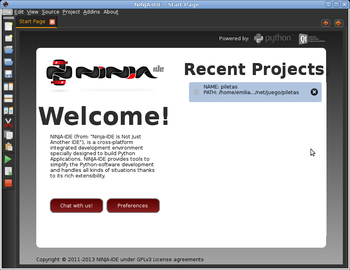
\includegraphics{files/img/u1/ninja-ide.png}
\end{figure}

Una lista bastante completa sobre las IDEs disponibles pueden
encontrarse en la \href{https://wiki.python.org/moin/IntegratedDevelopmentEnvironments}{wiki oficial de
Python}\footnote{https://wiki.python.org/moin/IntegratedDevelopmentEnvironments}


\section{Algoritmos computacionales}
\label{Unidad01:algoritmos-computacionales}
En forma simplificada, un programa o software es un conjunto de
instrucciones que la computadora puede ejecutar. Este procedimiento
formado por un conjunto de instrucciones es lo que denominamos algoritmo
computacional. Una analogía a un algoritmo computacional es una receta
de cocina, por ejemplo:

\begin{Verbatim}[commandchars=\\\{\}]
Prender el fuego
Salar la carne
Controlar cada 5 minutos hasta que haya brasas
Poner la carne a la parrilla
Cocinar hasta que esté la carne, controlar cada 5 minutos
Dar vuelta la carne
Cocinar hasta que esté la carne, controlar cada 5 minutos
Si falta sal al probar, salar
\end{Verbatim}

En esta receta se ven una serie de instrucciones que deben ser seguidas
en un determinado orden, en algunos casos contamos con ingredientes,
intrucciones, decisiones y acciones que se repiten. No muy distinto a un
programa de computación, comencemos con algunos \emph{ingredientes} simples
de Python y veamos lo que podemos hacer con ellos.


\subsection{El primer programa}
\label{Unidad01:el-primer-programa}
El acercamiento inicial a un lenguaje de programación suele ser con el
archiconocido programa ``Hola mundo''. Consiste simmplemente en un
programa que muestra en pantalla ese mensaje.

Renunciando a cualquier pretención de originalidad comenzaremos del
mismo modo, pero despidiéndonos. Para esto utilizaremos la instrucción
\emph{print()} pasando el mensaje de despedida entre comillas, a continuación
la instrucción.

\begin{Verbatim}[commandchars=\\\{\}]
\PYG{k}{print}\PYG{p}{(}\PYG{l+s}{\PYGZdq{}}\PYG{l+s}{Adios mundo cruel!}\PYG{l+s}{\PYGZdq{}}\PYG{p}{)}
\end{Verbatim}

Podemos probar la intrucción directamente desde el intérprete, creando
con un editor de texto plano un archivo guardado como \code{chau.py} y
luego ejecutándolo desde la terminal haciendo \code{python3 chau.py}, o
bien utilizando un IDE y haciendo todo desde ahí mismo.

Ahora bien, es muchísimo más lo que podemos hacer programando además de
saludar cordialmente. Veamos los elementos de un programa que nos
permitirán realizar tareas más complejas y entretenidas.


\section{Modos de ejecutar tus programas}
\label{Unidad01:modos-de-ejecutar-tus-programas}
El intérprete interactivo de Python es una gran ayuda para realizar
pruebas y experimentar en tiempo real sobre el lenguaje. Sin embargo,
cuando cerramos el intérprete perdemos lo escrito, por lo que no es una
solución para escribir programas mas largos y con mayores complejidades.
Por otro lado, tampoco resulta poco práctico abrir el IDE para correr un
script Python. Entonces, para un programa guardado con el nombre
hola\_mundo.py, lo podemos ejecutar de las siguientes maneras:


\subsection{Desde la línea de comandos}
\label{Unidad01:desde-la-linea-de-comandos}
Abriendo una terminal, e invocando al intérprete python y luego la ruta
y nombre del archivo:

\begin{Verbatim}[commandchars=\\\{\}]
\PYGZdl{}python3 hola\PYGZus{}mundo.py
\end{Verbatim}


\subsection{Como un script}
\label{Unidad01:como-un-script}
Es posible ejecutarlo sin invocar al intérprete desde la línea de
comandos, para esto, se debe incluir al principio del programa la
siguiente línea:

\begin{Verbatim}[commandchars=\\\{\}]
\PYG{c}{\PYGZsh{}!/usr/bin/env python3}
\end{Verbatim}

Con esa línea, estaremos especificando en el mismo programa la ruta del
intérprete que debe ejecutarlo. Antes de poder ejecutarlo, debemos
otorgarle permisos de ejecución con el comando del sistema operativo
chmod:

\begin{Verbatim}[commandchars=\\\{\}]
\PYGZdl{}chmod +x hola\PYGZus{}mundo.py
\end{Verbatim}

Una vez realizado lo anterior, es posible ejecutarlo desde la terminal,
como cualquier ejecutable del sistema operativo, llamándolo con el
nombre del programa antecediendo ''./'' (punto barra, sin comillas):

\begin{Verbatim}[commandchars=\\\{\}]
\PYGZdl{}./hola\PYGZus{}mundo.py
Adiós mundo cruel
\end{Verbatim}


\section{Elementos de un programa}
\label{Unidad01:elementos-de-un-programa}
A continuación veremos los ingredientes fundamentales de un lenguaje de
programación como Python, para llevar a cabo los ejemplos utilizaremos
el intérprete interactivo mejorado ipython.


\subsection{Números y expresiones}
\label{Unidad01:numeros-y-expresiones}
Frecuentemente requerimos resolver cálculos matemáticos, las operaciones
aritméticas básicas son:
\begin{itemize}
\item {} 
adición: +

\item {} 
sustracción: -

\item {} 
multiplicación: *

\item {} 
división: /

\item {} 
módulo: \%

\item {} 
potencia: **

\item {} 
división entera: //

\end{itemize}

Las operaciones se pueden agrupar con paréntesis y tienen precedencia
estándar. Veamos unos ejemplos.

\begin{Verbatim}[commandchars=\\\{\}]
In [9]: 1/3
Out[9]: 0.3333333333333333

In [10]: 1//3
Out[10]: 0

In [11]: 10\PYGZpc{}3
Out[11]: 1

In [12]: 4\PYGZpc{}2
Out[12]: 0
\end{Verbatim}

El caso de la potencia, también nos sirve para calcular raices. Veamos
una potencia al cubo y luego una raíz cuadrada, equivalente a una
potencia a la 1/2.

\begin{Verbatim}[commandchars=\\\{\}]
In [13]: 5**3
Out[13]: 125

In [14]: 2**(1/2)
Out[14]: 1.4142135623730951
\end{Verbatim}

Los datos numéricos obtenidos en las operaciones previas se clasifican
en reales y enteros, en python se los clasifica como float e int
respectivamente, además existe el tipo complex, para números complejos.

Utilizando la función type() podemos identificar el tipo de dato.
Veamos:

\begin{Verbatim}[commandchars=\\\{\}]
In [15]: type(0.333)
Out[15]: float

In [16]: type(4)
Out[16]: int
\end{Verbatim}


\subsection{Cadenas de carateres}
\label{Unidad01:cadenas-de-carateres}
Además de números, es posible manipular texto. Las cadenas son
secuencias de caracteres encerradas en comillas simples (`...') o dobles
(''...''), el tipo de datos es denominado \emph{str} (string). Sin adentrarnos
en detalles, que posteriormente veremos, aquí trataremos lo
indispensable para poder desarrollar los primeros programas. Veamos unos
ejemplos:

\begin{Verbatim}[commandchars=\\\{\}]
\PYG{g+gp}{\PYGZgt{}\PYGZgt{}\PYGZgt{} }\PYG{l+s}{\PYGZsq{}}\PYG{l+s}{huevos y pan}\PYG{l+s}{\PYGZsq{}}         \PYG{c}{\PYGZsh{} comillas simples}
\PYG{g+go}{\PYGZsq{}huevos y pan\PYGZsq{}}
\end{Verbatim}

Los operadores algebraicos para la suma y multiplicación tienen efecto
sobre las cadenas:

\begin{Verbatim}[commandchars=\\\{\}]
\PYG{g+gp}{\PYGZgt{}\PYGZgt{}\PYGZgt{} }\PYG{l+s}{\PYGZsq{}}\PYG{l+s}{eco }\PYG{l+s}{\PYGZsq{}}\PYG{o}{*}\PYG{l+m+mi}{4}               \PYG{c}{\PYGZsh{} La multiplicación repite la cadena}
\PYG{g+go}{\PYGZsq{}eco eco eco eco \PYGZsq{}}

\PYG{g+go}{\PYGZgt{}\PYGZgt{}\PYGZgt{}\PYGZsq{}yo y \PYGZsq{}+ \PYGZsq{}mi otro yo\PYGZsq{}   \PYGZsh{} La suma concatena dos o mas cadenas}
\PYG{g+go}{\PYGZsq{}yo y mi otro yo\PYGZsq{}}
\end{Verbatim}

Es posible utilizar cadenas de más de una línea, anteponiendo \textbf{triples
comillas} simples o dobles al inicio y al final, por ejemplo (fragmento
del poema de Fortunato Ramos \emph{Yo jamás fui un niño}):

\begin{Verbatim}[commandchars=\\\{\}]
\PYG{l+s+sd}{\PYGZsq{}\PYGZsq{}\PYGZsq{}}
\PYG{l+s+sd}{Mi sonrisa es seca y mi rostro es serio,}
\PYG{l+s+sd}{mis espaldas anchas, mis músculos duros}
\PYG{l+s+sd}{mis manos partidas por el crudo frío}
\PYG{l+s+sd}{sólo ocho años tengo, pero no soy un niño.}
\PYG{l+s+sd}{\PYGZsq{}\PYGZsq{}\PYGZsq{}}
\end{Verbatim}


\subsection{Comentarios}
\label{Unidad01:comentarios}
En los ejemplos previos y siguientes, veremos dentro del código
comentarios explicativos que no serán ejecutados por el intérprete. Su
uso solamente está destinado a quien lea el código, como texto
explicativo para orientar sobre lo que se realiza.

Los comentarios pueden ser de una única o múltiples líneas. Para el
primer caso se utiliza el símbolo numeral. Lo que continúa a la derecha
de su uso no es ejecutado.

Los comentarios de múltiples líneas se deben escribir entre triples
comillas, ya sean simples o dobles.


\subsection{Variables}
\label{Unidad01:variables}
Las variables son contenedores para almacenar información. Por ejemplo,
para elevar un número al cubo podemos utilizar 3 variables, para la base
(\emph{num1}), para el exponenete (\emph{num2}) y para almacenar el \emph{resultado}:

\begin{Verbatim}[commandchars=\\\{\}]
\PYG{n}{num1} \PYG{o}{=} \PYG{l+m+mi}{5}                   \PYG{c}{\PYGZsh{} num1 toma valor 5.}
\PYG{n}{num2} \PYG{o}{=} \PYG{l+m+mi}{3}                   \PYG{c}{\PYGZsh{} num2 toma 3.}
\PYG{n}{resultado} \PYG{o}{=} \PYG{n}{num1}\PYG{o}{*}\PYG{o}{*}\PYG{n}{num2}     \PYG{c}{\PYGZsh{} resultado toma num1 elevado a num2.}
\PYG{k}{print}\PYG{p}{(}\PYG{l+s}{\PYGZsq{}}\PYG{l+s}{El resultado es}\PYG{l+s}{\PYGZsq{}}\PYG{p}{,} \PYG{n}{resultado}\PYG{p}{)}
\end{Verbatim}

El operador igual (=) sirve para asignar lo que está a su derecha, a la
variable que se encuentra a su izquierda. Implementemos la siguiente
ecuación para dos valores de \emph{x}, 0.1 y 0.2.
\begin{gather}
\begin{split}y = (x-4)^2-3\end{split}\notag
\end{gather}
\begin{Verbatim}[commandchars=\\\{\}]
\PYG{n}{x1} \PYG{o}{=} \PYG{l+m+mf}{0.1}
\PYG{n}{y1} \PYG{o}{=} \PYG{p}{(}\PYG{n}{x1}\PYG{o}{\PYGZhy{}}\PYG{l+m+mi}{4}\PYG{p}{)}\PYG{o}{*}\PYG{o}{*}\PYG{l+m+mi}{2}\PYG{o}{\PYGZhy{}}\PYG{l+m+mi}{3}

\PYG{n}{x2} \PYG{o}{=} \PYG{l+m+mf}{0.2}
\PYG{n}{y2} \PYG{o}{=} \PYG{p}{(}\PYG{n}{x2}\PYG{o}{\PYGZhy{}}\PYG{l+m+mi}{4}\PYG{p}{)}\PYG{o}{*}\PYG{o}{*}\PYG{l+m+mi}{2}\PYG{o}{\PYGZhy{}}\PYG{l+m+mi}{3}

\PYG{k}{print}\PYG{p}{(}\PYG{n}{x1}\PYG{p}{,}\PYG{n}{y1}\PYG{p}{)}
\PYG{k}{print}\PYG{p}{(}\PYG{n}{x2}\PYG{p}{,}\PYG{n}{y2}\PYG{p}{)}
\end{Verbatim}

Veremos la siguiente salida por pantalla:

\begin{Verbatim}[commandchars=\\\{\}]
0.1 12.209999999999999
0.2 11.44
\end{Verbatim}

Otros ejemplos utilizando variables que contengan \textbf{cadenas de
caracteres}:

\begin{Verbatim}[commandchars=\\\{\}]
\PYG{n}{cadena1} \PYG{o}{=} \PYG{l+s}{\PYGZsq{}}\PYG{l+s}{siento que }\PYG{l+s}{\PYGZsq{}}
\PYG{n}{cadena2} \PYG{o}{=} \PYG{l+s}{\PYGZsq{}}\PYG{l+s}{nací en el viento }\PYG{l+s}{\PYGZsq{}}

\PYG{n}{cadena3} \PYG{o}{=} \PYG{n}{cadena1} \PYG{o}{+} \PYG{n}{cadena2}

\PYG{k}{print}\PYG{p}{(}\PYG{n}{cadena3}\PYG{p}{)}
\end{Verbatim}

Los nombres de las variables (identificador o etiqueta) pueden estar
formados por letras, dígitos y guiones bajos, teniendo en cuenta ciertas
restricciones, no pueden comenzar con un número y ni ser algunas de las
siguientes palabras reservadas:

\begin{Verbatim}[commandchars=\\\{\}]
False      class      finally    is         return
None       continue   for        lambda     try
True       def        from       nonlocal   while
and        del        global     not        with
as         elif       if         or         yield
assert     else       import     pass
break      except     in         raise
\end{Verbatim}

Se debe tener en cuenta que las variables diferencian entre mayúsculas y
minúsculas, de modo que juana, JUANA, JuAnA, JUANa son variables
diferentes. Esta característica suele denominarse como \emph{case-sensitive}.


\subsection{Lectura de datos}
\label{Unidad01:lectura-de-datos}
De los ejemplos que vimos, los valores que almacenan las variables
fueron ingresados en el mismo código, difícilmente sea útil contar con
los valores cargados en el programa en forma estática. Por esta razón,
generalmente se requiere leer información de diferentes fuentes, puede
ser desde un archivo o bien interactuando con un usuario.

La lectura de datos desde el teclado se realiza utilizando la sentencia
\emph{input()} del siguiente modo:

\begin{Verbatim}[commandchars=\\\{\}]
\PYG{n}{nombre} \PYG{o}{=} \PYG{n+nb}{input}\PYG{p}{(}\PYG{l+s}{\PYGZdq{}}\PYG{l+s}{¿Cómo es su nombre, maestro? }\PYG{l+s}{\PYGZdq{}}\PYG{p}{)}
\PYG{k}{print} \PYG{l+s}{\PYGZdq{}}\PYG{l+s}{Hola, }\PYG{l+s}{\PYGZdq{}} \PYG{o}{+} \PYG{n}{nombre} \PYG{o}{+} \PYG{l+s}{\PYGZdq{}}\PYG{l+s}{!}\PYG{l+s}{\PYGZdq{}}
\end{Verbatim}

El comportamiento es:

\begin{Verbatim}[commandchars=\\\{\}]
¿Cómo es su nombre, maestro?
Juan de los palotes
Hola, Juan de los palotes!
\end{Verbatim}

Es importante tener en cuenta que toda lectura por teclado utilizando la
función \emph{input()} va a almacenar lo ingresado como una variable de tipo
\emph{str}, es decir una cadena de caracteres. Veamos el comportamiento al
sumar dos números:

\begin{Verbatim}[commandchars=\\\{\}]
\PYG{n}{num1} \PYG{o}{=} \PYG{n+nb}{input}\PYG{p}{(}\PYG{l+s}{\PYGZdq{}}\PYG{l+s}{Ingrese un número = }\PYG{l+s}{\PYGZdq{}}\PYG{p}{)}
\PYG{n}{num2} \PYG{o}{=} \PYG{n+nb}{input}\PYG{p}{(}\PYG{l+s}{\PYGZdq{}}\PYG{l+s}{Ingrese otro número = }\PYG{l+s}{\PYGZdq{}}\PYG{p}{)}
\PYG{k}{print}\PYG{p}{(}\PYG{l+s}{\PYGZdq{}}\PYG{l+s}{El resultado es =}\PYG{l+s}{\PYGZdq{}}\PYG{p}{,} \PYG{n}{num1}\PYG{o}{+}\PYG{n}{num2}\PYG{p}{)}
\end{Verbatim}

\begin{Verbatim}[commandchars=\\\{\}]
Ingrese un número = 28
Ingrese otro número = 03
El resultado es = 2803
\end{Verbatim}

Claramente la suma de los valores ingresados no da el resultado
observado. El inconveniente se debe a que ambos valores son tomados como
cadenas de caracteres y la operación de suma entre cadenas de caracteres
produce la concatenación de las mismas. Es necesaria convertir la cadena
de caracteres (str) a un valor numérico, ya sea entero o real (int o
float).

Para convertir datos de diferentes tipo se utilizan las funciones int(),
float() o str(). Modificando el caso anterior:

\begin{Verbatim}[commandchars=\\\{\}]
\PYG{n}{num1} \PYG{o}{=} \PYG{n+nb}{int}\PYG{p}{(}\PYG{n+nb}{input}\PYG{p}{(}\PYG{l+s}{\PYGZdq{}}\PYG{l+s}{Ingrese un número = }\PYG{l+s}{\PYGZdq{}}\PYG{p}{)}\PYG{p}{)}
\PYG{n}{num2} \PYG{o}{=} \PYG{n+nb}{int}\PYG{p}{(}\PYG{n+nb}{input}\PYG{p}{(}\PYG{l+s}{\PYGZdq{}}\PYG{l+s}{Ingrese otro número = }\PYG{l+s}{\PYGZdq{}}\PYG{p}{)}\PYG{p}{)}
\PYG{k}{print}\PYG{p}{(}\PYG{l+s}{\PYGZdq{}}\PYG{l+s}{El resultado es =}\PYG{l+s}{\PYGZdq{}}\PYG{p}{,} \PYG{n}{num1}\PYG{o}{+}\PYG{n}{num2}\PYG{p}{)}
\end{Verbatim}

\begin{Verbatim}[commandchars=\\\{\}]
Ingrese un número = 28
Ingrese otro número = 03
El resultado es = 31
\end{Verbatim}

Veamos un ejemplo para operar directamente el valor leído en una
ecuación matemática con el siguiente código:

\begin{Verbatim}[commandchars=\\\{\}]
\PYG{n}{x} \PYG{o}{=} \PYG{n+nb}{input}\PYG{p}{(}\PYG{l+s}{\PYGZdq{}}\PYG{l+s}{Ingrese x = }\PYG{l+s}{\PYGZdq{}}\PYG{p}{)}
\PYG{n}{y} \PYG{o}{=} \PYG{p}{(}\PYG{n}{x}\PYG{o}{\PYGZhy{}}\PYG{l+m+mi}{4}\PYG{p}{)}\PYG{o}{*}\PYG{o}{*}\PYG{l+m+mi}{2}\PYG{o}{\PYGZhy{}}\PYG{l+m+mi}{3}
\PYG{k}{print}\PYG{p}{(}\PYG{n}{x}\PYG{p}{,}\PYG{n}{y}\PYG{p}{)}
\end{Verbatim}

\begin{Verbatim}[commandchars=\\\{\}]
Ingrese x = 3
\end{Verbatim}

\begin{Verbatim}[commandchars=\\\{\}]
\PYGZhy{}\PYGZhy{}\PYGZhy{}\PYGZhy{}\PYGZhy{}\PYGZhy{}\PYGZhy{}\PYGZhy{}\PYGZhy{}\PYGZhy{}\PYGZhy{}\PYGZhy{}\PYGZhy{}\PYGZhy{}\PYGZhy{}\PYGZhy{}\PYGZhy{}\PYGZhy{}\PYGZhy{}\PYGZhy{}\PYGZhy{}\PYGZhy{}\PYGZhy{}\PYGZhy{}\PYGZhy{}\PYGZhy{}\PYGZhy{}\PYGZhy{}\PYGZhy{}\PYGZhy{}\PYGZhy{}\PYGZhy{}\PYGZhy{}\PYGZhy{}\PYGZhy{}\PYGZhy{}\PYGZhy{}\PYGZhy{}\PYGZhy{}\PYGZhy{}\PYGZhy{}\PYGZhy{}\PYGZhy{}\PYGZhy{}\PYGZhy{}\PYGZhy{}\PYGZhy{}\PYGZhy{}\PYGZhy{}\PYGZhy{}\PYGZhy{}\PYGZhy{}\PYGZhy{}\PYGZhy{}\PYGZhy{}\PYGZhy{}\PYGZhy{}\PYGZhy{}\PYGZhy{}\PYGZhy{}\PYGZhy{}\PYGZhy{}\PYGZhy{}\PYGZhy{}\PYGZhy{}\PYGZhy{}\PYGZhy{}\PYGZhy{}\PYGZhy{}\PYGZhy{}\PYGZhy{}\PYGZhy{}\PYGZhy{}\PYGZhy{}\PYGZhy{}
TypeError                                 Traceback (most recent call last)

\PYGZlt{}ipython\PYGZhy{}input\PYGZhy{}15\PYGZhy{}3baa5c95d16e\PYGZgt{} in \PYGZlt{}module\PYGZgt{}()
      1 x = input(\PYGZdq{}Ingrese x = \PYGZdq{})
\PYGZhy{}\PYGZhy{}\PYGZhy{}\PYGZhy{}\PYGZgt{} 2 y = (x\PYGZhy{}4)**2\PYGZhy{}3
      3 print(x,y)


TypeError: unsupported operand type(s) for \PYGZhy{}: \PYGZsq{}str\PYGZsq{} and \PYGZsq{}int\PYGZsq{}
\end{Verbatim}

A diferencia del ejemplo visto anteriormente, donde la suma de dos
cadenas era una operación perfectamente válida, ahora nos encontramos
con operaciones entre diferentes tipos pero incompatibles. En este caso,
podemos convertir la entrada en un número flotante para opearar con
normalidad:

\begin{Verbatim}[commandchars=\\\{\}]
\PYG{n}{x} \PYG{o}{=} \PYG{n+nb}{float}\PYG{p}{(}\PYG{n+nb}{input}\PYG{p}{(}\PYG{l+s}{\PYGZdq{}}\PYG{l+s}{Ingrese x = }\PYG{l+s}{\PYGZdq{}}\PYG{p}{)}\PYG{p}{)}
\PYG{n}{y} \PYG{o}{=} \PYG{p}{(}\PYG{n}{x}\PYG{o}{\PYGZhy{}}\PYG{l+m+mi}{4}\PYG{p}{)}\PYG{o}{*}\PYG{o}{*}\PYG{l+m+mi}{2}\PYG{o}{\PYGZhy{}}\PYG{l+m+mi}{3}
\PYG{k}{print}\PYG{p}{(}\PYG{n}{x}\PYG{p}{,}\PYG{n}{y}\PYG{p}{)}
\end{Verbatim}

\begin{Verbatim}[commandchars=\\\{\}]
Ingrese x = 3
3.0 \PYGZhy{}2.0
\end{Verbatim}

Es posible combinar distintos tipos de datos haciendo la conversión
correspondiente, en el último ejemplo, tanto \emph{x} como \emph{y} son de tipo
\emph{float} y es posible concatenarlos a una cadena de caracteres haciendo
la conversión correspondiente, utilizando la función \emph{str()}:

\begin{Verbatim}[commandchars=\\\{\}]
\PYG{n}{mensaje} \PYG{o}{=} \PYG{l+s}{\PYGZsq{}}\PYG{l+s}{y vale }\PYG{l+s}{\PYGZsq{}} \PYG{o}{+} \PYG{n+nb}{str}\PYG{p}{(}\PYG{n}{y}\PYG{p}{)} \PYG{o}{+} \PYG{l+s}{\PYGZsq{}}\PYG{l+s}{ para un valor de x = }\PYG{l+s}{\PYGZsq{}}\PYG{o}{+} \PYG{n+nb}{str}\PYG{p}{(}\PYG{n}{x}\PYG{p}{)}
\end{Verbatim}


\subsection{Escritura de datos}
\label{Unidad01:escritura-de-datos}
Hemos hecho uso de la función \emph{print()} en su mínima expresión. Iremos
viendo diferentes usos a partir de las siguientes variables:

\begin{Verbatim}[commandchars=\\\{\}]
\PYG{c}{\PYGZsh{} Variables a imprimir}
\PYG{n}{cad} \PYG{o}{=} \PYG{l+s}{\PYGZsq{}}\PYG{l+s}{Pi es}\PYG{l+s}{\PYGZsq{}}
\PYG{n}{pi} \PYG{o}{=} \PYG{l+m+mf}{3.1415}
\PYG{n}{mil} \PYG{o}{=} \PYG{l+m+mi}{1000}
\PYG{n}{uno} \PYG{o}{=} \PYG{l+m+mi}{1}
\end{Verbatim}


\subsubsection{Como argumentos}
\label{Unidad01:como-argumentos}
La forma más simple es separar los argumentos a ser impresos mediante
comas.

\begin{Verbatim}[commandchars=\\\{\}]
\PYG{k}{print}\PYG{p}{(}\PYG{n}{cad}\PYG{p}{,}\PYG{n}{pi}\PYG{p}{,}\PYG{l+s}{\PYGZsq{}}\PYG{l+s}{aproximadamente}\PYG{l+s}{\PYGZsq{}}\PYG{p}{)}
\end{Verbatim}

\begin{Verbatim}[commandchars=\\\{\}]
Pi es 3.1415 aproximadamente
\end{Verbatim}

Por defecto, la separación que se obtiene entre cada argumento es un
espacio en blanco, sin embargo, se puede cambiar este comportamiento
agregando como argumento \textbf{*sep=' `*} y entre las comillas incluir el
separador deseado, por ejemplo:

\begin{Verbatim}[commandchars=\\\{\}]
print(cad,pi,\PYGZsq{}aproximadamente\PYGZsq{}, sep=\PYGZsq{};\PYGZsq{})
print(cad,pi,\PYGZsq{}aproximadamente\PYGZsq{}, sep=\PYGZsq{},\PYGZsq{})
print(cad,pi,\PYGZsq{}aproximadamente\PYGZsq{}, sep=\PYGZsq{}:\PYGZhy{})\PYGZsq{})
\end{Verbatim}

\begin{Verbatim}[commandchars=\\\{\}]
Pi es;3.1415;aproximadamente
Pi es,3.1415,aproximadamente
Pi es:\PYGZhy{})3.1415:\PYGZhy{})aproximadamente
\end{Verbatim}

Como vemos, en cada ejecución la impresión se realiza en diferentes
renglones, este es el comportamiento por defecto, que puede ser
modificando agregando el parámetro \textbf{*end='' ``*}. Reflejemos esto con un
ejemplo:

\begin{Verbatim}[commandchars=\\\{\}]
print(1, end=\PYGZdq{} \PYGZdq{})
print(2, end=\PYGZdq{} \PYGZdq{})
print(3)
print(4)
\end{Verbatim}

\begin{Verbatim}[commandchars=\\\{\}]
1 2 3
4
\end{Verbatim}


\subsubsection{Usando comodines}
\label{Unidad01:usando-comodines}
Los comodines consisten en una marca especial en la cadena a imprimir
que es reemplazada por la variable y el formato que se le indique.
Existen tres tipos de comodines, para números enteros, reales
(flotantes) y para cadenas de caracteres:
\begin{itemize}
\item {} 
Comodín para reales: \%f

\item {} 
Comodín para enteros: \%d

\item {} 
Comodín para cadenas: \%s

\end{itemize}

Se utilizan del siguiente modo:

\begin{Verbatim}[commandchars=\\\{\}]
\PYG{k}{print}\PYG{p}{(}\PYG{l+s}{\PYGZsq{}}\PYG{l+s}{Pi es }\PYG{l+s+si}{\PYGZpc{}f}\PYG{l+s}{ aproximadamente}\PYG{l+s}{\PYGZsq{}} \PYG{o}{\PYGZpc{}}\PYG{n}{pi}\PYG{p}{)}
\PYG{k}{print}\PYG{p}{(}\PYG{l+s}{\PYGZsq{}}\PYG{l+s}{El número }\PYG{l+s+si}{\PYGZpc{}d}\PYG{l+s}{ es }\PYG{l+s+si}{\PYGZpc{}s}\PYG{l+s}{ que }\PYG{l+s+si}{\PYGZpc{}d}\PYG{l+s}{\PYGZsq{}} \PYG{o}{\PYGZpc{}}\PYG{p}{(}\PYG{n}{mil}\PYG{p}{,}\PYG{l+s}{\PYGZdq{}}\PYG{l+s}{menor}\PYG{l+s}{\PYGZdq{}}\PYG{p}{,}\PYG{n}{mil}\PYG{o}{\PYGZhy{}}\PYG{l+m+mi}{1}\PYG{p}{)}\PYG{p}{)}
\end{Verbatim}

\begin{Verbatim}[commandchars=\\\{\}]
Pi es 3.141500 aproximadamente
El número 1000 es menor que 999
\end{Verbatim}

Es posible formatear los valores, elegir el ancho del campo, la cantidad
de decimales, entre muchas otras funciones.

\begin{Verbatim}[commandchars=\\\{\}]
\PYG{k}{print}\PYG{p}{(}\PYG{l+s}{\PYGZsq{}}\PYG{l+s+si}{\PYGZpc{}.2f}\PYG{l+s}{ }\PYG{l+s+si}{\PYGZpc{}.4f}\PYG{l+s}{ }\PYG{l+s+si}{\PYGZpc{}.3f}\PYG{l+s}{\PYGZsq{}} \PYG{o}{\PYGZpc{}}\PYG{p}{(}\PYG{n}{pi}\PYG{p}{,}\PYG{n}{pi}\PYG{p}{,}\PYG{n}{pi}\PYG{p}{)}\PYG{p}{)}
\PYG{k}{print}\PYG{p}{(}\PYG{l+s}{\PYGZsq{}}\PYG{l+s+si}{\PYGZpc{}4d}\PYG{l+s}{\PYGZsq{}} \PYG{o}{\PYGZpc{}}\PYG{n}{uno}\PYG{p}{)}
\end{Verbatim}

\begin{Verbatim}[commandchars=\\\{\}]
\PYGZhy{}\PYGZhy{}\PYGZhy{}\PYGZhy{}\PYGZhy{}\PYGZhy{}\PYGZhy{}\PYGZhy{}\PYGZhy{}\PYGZhy{}\PYGZhy{}\PYGZhy{}\PYGZhy{}\PYGZhy{}\PYGZhy{}\PYGZhy{}\PYGZhy{}\PYGZhy{}\PYGZhy{}\PYGZhy{}\PYGZhy{}\PYGZhy{}\PYGZhy{}\PYGZhy{}\PYGZhy{}\PYGZhy{}\PYGZhy{}\PYGZhy{}\PYGZhy{}\PYGZhy{}\PYGZhy{}\PYGZhy{}\PYGZhy{}\PYGZhy{}\PYGZhy{}\PYGZhy{}\PYGZhy{}\PYGZhy{}\PYGZhy{}\PYGZhy{}\PYGZhy{}\PYGZhy{}\PYGZhy{}\PYGZhy{}\PYGZhy{}\PYGZhy{}\PYGZhy{}\PYGZhy{}\PYGZhy{}\PYGZhy{}\PYGZhy{}\PYGZhy{}\PYGZhy{}\PYGZhy{}\PYGZhy{}\PYGZhy{}\PYGZhy{}\PYGZhy{}\PYGZhy{}\PYGZhy{}\PYGZhy{}\PYGZhy{}\PYGZhy{}\PYGZhy{}\PYGZhy{}\PYGZhy{}\PYGZhy{}\PYGZhy{}\PYGZhy{}\PYGZhy{}\PYGZhy{}\PYGZhy{}\PYGZhy{}\PYGZhy{}\PYGZhy{}

NameError                                 Traceback (most recent call last)

\PYGZlt{}ipython\PYGZhy{}input\PYGZhy{}1\PYGZhy{}f45a2755e54d\PYGZgt{} in \PYGZlt{}module\PYGZgt{}()
\PYGZhy{}\PYGZhy{}\PYGZhy{}\PYGZhy{}\PYGZgt{} 1 print(\PYGZsq{}\PYGZpc{}.2f \PYGZpc{}.4f \PYGZpc{}.3f\PYGZsq{} \PYGZpc{}(pi,pi,pi))
      2 print(\PYGZsq{}\PYGZpc{}4d\PYGZsq{} \PYGZpc{}uno)


NameError: name \PYGZsq{}pi\PYGZsq{} is not defined
\end{Verbatim}

La sintaxis general del uso de comodines es:

\begin{Verbatim}[commandchars=\\\{\}]
\PYGZpc{}[opciones][ancho][.precisión]tipo
\end{Verbatim}

Algunas variantes de lo visto se explica en la siguiente lista:
\begin{itemize}
\item {} 
\%d : un entero

\item {} 
\%5d: un entero escrito en un campo de 5 caracteres, alineado a la
derecha

\item {} 
\%-5d: un entero escrito en un campo de 5 caracteres, alineado a la
izquierda

\item {} 
\%05d: un entero escrito en un campo de 5 caracteres, completado con
ceros desde la izquierda (ej. 00041)

\item {} 
\%e: flotante escrito en notación científica

\item {} 
\%E: como \%e, pero E en mayúscula

\item {} 
\%11.3e: flotante escrito en notación científica con 3 decimales en un
campo de 11 caracteres

\item {} 
\%.3e: flotante escrito en notación científica con 3 decimales en un
campo de ancho mínimo

\item {} 
\%5.1f: flotante con un decimal en un campo de 5 de caracteres

\item {} 
\%.3f: flotante con 3 decimales en un campo de mínimo ancho

\item {} 
\%s: una cadena

\item {} 
\%-20s: una cadena alineada a la izquierda en un campo de 20
caracteres de ancho

\end{itemize}

Con lo visto hasta aquí tenemos suficientes alternativas para mostrar en
pantalla información de diferentes tipos. Existen una alternativa para
imprimir en pantalla utilizando el método format, el lector interesado
puede indagar más al respecto en
\href{http://docs.python.org.ar/tutorial/3/inputoutput.html}{http://docs.python.org.ar/tutorial/3/inputoutput.html} , en el capítulo
Entrada y Salida del tutorial de Python oficial
\href{http://docs.python.org.ar/tutorial/pdfs/TutorialPython3.pdf}{http://docs.python.org.ar/tutorial/pdfs/TutorialPython3.pdf} ó también en
\href{http://www.python-course.eu/python3\_formatted\_output.php}{http://www.python-course.eu/python3\_formatted\_output.php}


\subsection{Operadores relacionales y lógicos}
\label{Unidad01:operadores-relacionales-y-logicos}
¿¿¿capaz va a la unidad siguiente!!! - Coincido :D


\subsection{Funciones}
\label{Unidad01:funciones}
Las funciones son programas o subprogramas que realizan una determinada
acción y pueden ser invocados desde otro programa. En los capítulos
posteriores trabajaremos intensamente con funciones creando propias, sin
embargo en esta sección, con el fin de comprender su uso, presentaremos
algunas pocas de las que nos provee Python.

El uso de funciones nativas en Python es directo, veamos algunas:

\begin{Verbatim}[commandchars=\\\{\}]
\PYG{n}{frase} \PYG{o}{=} \PYG{l+s}{\PYGZsq{}}\PYG{l+s}{simple es mejor que complejo}\PYG{l+s}{\PYGZsq{}}
\PYG{n}{num\PYGZus{}letras} \PYG{o}{=} \PYG{n+nb}{len}\PYG{p}{(}\PYG{n}{frase}\PYG{p}{)}
\PYG{k}{print}\PYG{p}{(}\PYG{n}{num\PYGZus{}letras}\PYG{p}{)}
\end{Verbatim}

\begin{Verbatim}[commandchars=\\\{\}]
\PYG{l+m+mi}{28}
\end{Verbatim}

El ejemplo previo hicimos uso de dos funciones, por un lado la función
\textbf{*print()*}, presentada ya desde el primer programa y una nueva
función, \textbf{*len()*}, que recibe como dato de entrada una cadena de
caracteres y calcula la cantidad de caracteres de la misma y lo retorna
de manera tal que lo podemos asignar a una variable (num\_letras).

ver ejemplo 2-3 pág 38 de Begining Python from novice to professional
2nd edition.

Estos subprogramas pueden están vinculadas, de modo que se organizan en
módulos.


\subsection{Módulos}
\label{Unidad01:modulos}
Python posee cientos de funciones que se organizan o agrupan en módulos.
Veamos un ejemplo para calcular la raiz cuadrada, el seno y coseno de un
número haciendo uso de las funciones \emph{sqrt()}, \emph{sin()} y \emph{cos()}, todas
ubicadas bajo el módulo math.

\begin{Verbatim}[commandchars=\\\{\}]
\PYG{k+kn}{import} \PYG{n+nn}{math}

\PYG{n}{nro} \PYG{o}{=} \PYG{l+m+mi}{2}
\PYG{n}{raiz} \PYG{o}{=} \PYG{n}{math}\PYG{o}{.}\PYG{n}{sqrt}\PYG{p}{(}\PYG{n}{nro}\PYG{p}{)}
\PYG{k}{print}\PYG{p}{(}\PYG{l+s}{\PYGZdq{}}\PYG{l+s}{La raiz de }\PYG{l+s+si}{\PYGZpc{}d}\PYG{l+s}{ es }\PYG{l+s+si}{\PYGZpc{}.4f}\PYG{l+s}{\PYGZdq{}} \PYG{o}{\PYGZpc{}}\PYG{p}{(}\PYG{n}{nro}\PYG{p}{,}\PYG{n}{raiz}\PYG{p}{)}\PYG{p}{)}
\PYG{k}{print}\PYG{p}{(}\PYG{l+s}{\PYGZdq{}}\PYG{l+s}{El seno de }\PYG{l+s+si}{\PYGZpc{}d}\PYG{l+s}{ es }\PYG{l+s+si}{\PYGZpc{}.4f}\PYG{l+s}{\PYGZdq{}} \PYG{o}{\PYGZpc{}}\PYG{p}{(}\PYG{n}{nro}\PYG{p}{,}\PYG{n}{math}\PYG{o}{.}\PYG{n}{sin}\PYG{p}{(}\PYG{n}{nro}\PYG{p}{)}\PYG{p}{)}\PYG{p}{)}
\PYG{k}{print}\PYG{p}{(}\PYG{l+s}{\PYGZdq{}}\PYG{l+s}{El coseno de }\PYG{l+s+si}{\PYGZpc{}d}\PYG{l+s}{ es }\PYG{l+s+si}{\PYGZpc{}.4f}\PYG{l+s}{\PYGZdq{}} \PYG{o}{\PYGZpc{}}\PYG{p}{(}\PYG{n}{nro}\PYG{p}{,}\PYG{n}{math}\PYG{o}{.}\PYG{n}{cos}\PYG{p}{(}\PYG{n}{nro}\PYG{p}{)}\PYG{p}{)}\PYG{p}{)}
\end{Verbatim}

\begin{Verbatim}[commandchars=\\\{\}]
La raiz de 2 es 1.4142
El seno de 2 es 0.9093
El coseno de 2 es \PYGZhy{}0.4161
\end{Verbatim}

Del ejemplo previo, hemos visto como indicarle a Python que importe -o
haga uso de- un módulo en particular y de algunas de sus funciones
incluidas.

En capítulos posteriores veremos en profundidad distintos modos de
importar módulos e invocar sus funciones.


\section{Ejercicios}
\label{Unidad01:ejercicios}
1- Realice un programa que permita al usuario ingresar una temperatura
en grados centígrados y que muestre su equivalente en grados fahrenheit.

\begin{Verbatim}[commandchars=\\\{\}]
Ingrese temperatura en °C: 33.8
Conversión a Fahrenheit: 92.84
\end{Verbatim}

2- Realice un programa que permita al usuario ingresar su nombre y que
luego lo muestre repetido en pantalla tantas vees como cantidad de
letras posea el nombre.

3- Ingrese el nombre y edad de dos personas en variables separadas
(nom1, edad1, nom2, edad2). Luego, intercambie la edad y muestre el
resultado en pantalla. Indague de qué manera puede intercambiar el
contenido de variables en Python.

4- La simple tarea de realizar la cocción de un huevo pasado por agua
tiene sus secretos. Con la ecuación a continuación se puede conocer el
tiempo en alcanzar el punto exacto. Programe la ecuación para valores de
bla bla bla

5- Lea por teclado el valor del cuenta kilómetros de un automovil,
posteriormente, permita ingresar el nuevo valor luego de realizar un
viaje y muestre en pantalla los kilómetros recorridos, así como también
ese valor en metros, centímetros, yardas y pies.

6- Las benévolas companías telefónicas cobran la tarifa de cada llamada
del siguiente modo: un valor fijo de \$0.80 cuando se establece la
llamada, luego, fracciona por tiempo, donde el primer minuto tiene un
valor de \$1.30 y los subsiguientes de \$1.45. Realice un programa que
permita ingresar la duración de una llamada y que muestre luego el costo
total de la misma, a la que se le debe agregar un porcentaje del 20\%
correspondiente a impuestos.

7- Un atleta realiza sus entrenamientos para una maratón (42.195km) y
desea conocer su velocidad promedio. Desarrolle un programa donde se
ingrese el tiempo transcurrido en tres variables diferentes: horas,
minutos y segundos. Luego, muestre la velocidad promedio en km/h y
km/seg.

8- En el siguiente programa se calcula la diferencia de tiempo entre dos
marcas de tiempo. Analice el código del programa y explique las acciones
que se llevan a cabo. Luego, modifiquelo para que las dos marcas de
tiempo sean ingresadas por un usuario.

\begin{Verbatim}[commandchars=\\\{\}]
\PYG{c}{\PYGZsh{} dos marcas de tiempo}
\PYG{n}{hora1}\PYG{p}{,}\PYG{n}{min1}\PYG{p}{,}\PYG{n}{seg1} \PYG{o}{=} \PYG{l+m+mi}{14}\PYG{p}{,} \PYG{l+m+mi}{58}\PYG{p}{,}\PYG{l+m+mi}{59}
\PYG{n}{hora2}\PYG{p}{,}\PYG{n}{min2}\PYG{p}{,}\PYG{n}{seg2} \PYG{o}{=} \PYG{l+m+mi}{16}\PYG{p}{,} \PYG{l+m+mi}{0}\PYG{p}{,} \PYG{l+m+mi}{0}

\PYG{c}{\PYGZsh{} conversión del tiempo a segundos}
\PYG{n}{t1s} \PYG{o}{=} \PYG{n}{hora1}\PYG{o}{*}\PYG{l+m+mi}{60}\PYG{o}{*}\PYG{l+m+mi}{60} \PYG{o}{+} \PYG{n}{min1}\PYG{o}{*}\PYG{l+m+mi}{60} \PYG{o}{+} \PYG{n}{seg1}
\PYG{n}{t2s} \PYG{o}{=} \PYG{n}{hora2}\PYG{o}{*}\PYG{l+m+mi}{60}\PYG{o}{*}\PYG{l+m+mi}{60} \PYG{o}{+} \PYG{n}{min2}\PYG{o}{*}\PYG{l+m+mi}{60} \PYG{o}{+} \PYG{n}{seg2}

\PYG{c}{\PYGZsh{} diferencia}
\PYG{n}{t} \PYG{o}{=} \PYG{n+nb}{abs}\PYG{p}{(}\PYG{n}{t1s}\PYG{o}{\PYGZhy{}}\PYG{n}{t2s}\PYG{p}{)}

\PYG{c}{\PYGZsh{} cálculos de hora, minuto y segundos}
\PYG{n}{h} \PYG{o}{=} \PYG{n}{t}\PYG{o}{/}\PYG{o}{/}\PYG{l+m+mi}{3600}
\PYG{n}{m} \PYG{o}{=} \PYG{p}{(}\PYG{n}{t}\PYG{o}{\PYGZhy{}}\PYG{n}{h}\PYG{o}{*}\PYG{l+m+mi}{3600}\PYG{p}{)}\PYG{o}{/}\PYG{o}{/}\PYG{l+m+mi}{60}
\PYG{n}{s} \PYG{o}{=} \PYG{n}{t}\PYG{o}{\PYGZhy{}}\PYG{n}{h}\PYG{o}{*}\PYG{l+m+mi}{3600}\PYG{o}{\PYGZhy{}}\PYG{n}{m}\PYG{o}{*}\PYG{l+m+mi}{60}

\PYG{c}{\PYGZsh{} impresión en pantalla}
\PYG{k}{print} \PYG{p}{(}\PYG{l+s}{\PYGZsq{}}\PYG{l+s}{Diferencia de tiempo:}\PYG{l+s}{\PYGZsq{}}\PYG{p}{,} \PYG{n}{h}\PYG{p}{,} \PYG{l+s}{\PYGZsq{}}\PYG{l+s}{hs}\PYG{l+s}{\PYGZsq{}}\PYG{p}{,} \PYG{n}{m}\PYG{p}{,} \PYG{l+s}{\PYGZsq{}}\PYG{l+s}{min}\PYG{l+s}{\PYGZsq{}}\PYG{p}{,}\PYG{n}{s}\PYG{p}{,} \PYG{l+s}{\PYGZsq{}}\PYG{l+s}{seg}\PYG{l+s}{\PYGZsq{}}\PYG{p}{)}
\end{Verbatim}

\begin{Verbatim}[commandchars=\\\{\}]
\PYG{p}{(}\PYG{l+s}{\PYGZsq{}}\PYG{l+s}{Diferencia de tiempo:}\PYG{l+s}{\PYGZsq{}}\PYG{p}{,} \PYG{l+m+mi}{1}\PYG{p}{,} \PYG{l+s}{\PYGZsq{}}\PYG{l+s}{hs}\PYG{l+s}{\PYGZsq{}}\PYG{p}{,} \PYG{l+m+mi}{1}\PYG{p}{,} \PYG{l+s}{\PYGZsq{}}\PYG{l+s}{min}\PYG{l+s}{\PYGZsq{}}\PYG{p}{,} \PYG{l+m+mi}{1}\PYG{p}{,} \PYG{l+s}{\PYGZsq{}}\PYG{l+s}{seg}\PYG{l+s}{\PYGZsq{}}\PYG{p}{)}
\end{Verbatim}


\chapter{Tipos básicos}
\label{Unidad02::doc}\label{Unidad02:tipos-basicos}
Como vimos en la Unidad 1, las variables pueden contener diferentes
tipos de datos, y al ser distintos, son tratados de manera diferente por
Python (por ejemplo no podemos sumar un número con una letra).

Hemos visto 2 de los 3 tipos básicos que utiliza python, los cuales se
dividen en: * \textbf{Números} * \textbf{Cadenas de texto} * \textbf{Booleanos}


\section{Números}
\label{Unidad02:numeros}
Los números como vimos pueden ser enteros, reales (también denominados
de coma flotante) ó complejos. \#\#\# Enteros Los números enteros son
aquellos números positivos o negativos que no tienen decimales (además
del cero). En Python se pueden representar mediante el tipo int (de
integer, entero) o el tipo long (largo). La única diferencia es que el
tipo long permite almacenar números más grandes. Por ejemplo:

\begin{Verbatim}[commandchars=\\\{\}]
\PYG{n}{a} \PYG{o}{=} \PYG{l+m+mi}{4}
\PYG{n+nb}{type}\PYG{p}{(}\PYG{n}{a}\PYG{p}{)}
\end{Verbatim}

\begin{Verbatim}[commandchars=\\\{\}]
\PYG{n+nb}{int}
\end{Verbatim}

\begin{Verbatim}[commandchars=\\\{\}]
\PYG{n}{b} \PYG{o}{=} \PYG{l+m+mi+il}{28L}
\PYG{n+nb}{type}\PYG{p}{(}\PYG{n}{b}\PYG{p}{)}
\end{Verbatim}

\begin{Verbatim}[commandchars=\\\{\}]
\PYG{n+nb}{long}
\end{Verbatim}


\subsection{Reales}
\label{Unidad02:reales}
Los números reales son los que tienen decimales. En Python se expresan
mediante el tipo float.

Para representar un número real en Python se escribe primero la parte
entera, seguido de un punto y por último la parte decimal. Por ejemplo:

\begin{Verbatim}[commandchars=\\\{\}]
\PYG{n}{real} \PYG{o}{=} \PYG{l+m+mf}{6.2231}
\end{Verbatim}

También se puede utilizar notación científica, y añadir una e (de
exponente) para indicar un exponente en base 10. Por ejemplo:

\begin{Verbatim}[commandchars=\\\{\}]
\PYG{n}{real} \PYG{o}{=} \PYG{l+m+mf}{0.6e\PYGZhy{}3}
\end{Verbatim}

Lo que sería equivalente a 0.6 x 10-3 = 0.6 x 0.001 = 0.0006

\begin{Verbatim}[commandchars=\\\{\}]
\PYG{n}{real} \PYG{o}{=} \PYG{l+m+mf}{8.21}
\PYG{n+nb}{type}\PYG{p}{(}\PYG{n}{real}\PYG{p}{)}
\end{Verbatim}

\begin{Verbatim}[commandchars=\\\{\}]
\PYG{n+nb}{float}
\end{Verbatim}


\subsection{Complejos}
\label{Unidad02:complejos}
Los números complejos son aquellos que tienen parte imaginaria. Si no
conocías de su existencia, es más que probable que nunca lo vayas a
necesitar, de hecho la mayor parte de los lenguajes de programación
carecen de este tipo, aunque sea muy utilizado por ingenieros y
científicos en general.

En el caso de que necesites utilizar números complejos, debes saber que
son llamados complex en Python, y que se representan de la siguiente
forma:

\begin{Verbatim}[commandchars=\\\{\}]
\PYG{n}{c}\PYG{o}{=} \PYG{l+m+mi}{4} \PYG{o}{+} \PYG{l+m+mi}{5j}
\PYG{n+nb}{type}\PYG{p}{(}\PYG{n}{c}\PYG{p}{)}
\end{Verbatim}

\begin{Verbatim}[commandchars=\\\{\}]
\PYG{n+nb}{complex}
\end{Verbatim}


\section{Cadenas de texto}
\label{Unidad02:cadenas-de-texto}
Tal como hemos visto en la unidad anterior, las cadenas (string en
inglés ó str) no son más que texto encerrado entre comillas simples
(‘cadena’), dobles (“cadena”) ó triples(`'`Cadenas multilíneas'`'). Por
ejemplo:

\begin{Verbatim}[commandchars=\\\{\}]
\PYG{n}{a} \PYG{o}{=} \PYG{l+s}{\PYGZsq{}}\PYG{l+s}{El futuro mostrará los resultados y juzgará a cada uno de acuerdo a sus logros (Nikola Tesla)}\PYG{l+s}{\PYGZsq{}}
\PYG{n+nb}{type}\PYG{p}{(}\PYG{n}{a}\PYG{p}{)}
\end{Verbatim}

\begin{Verbatim}[commandchars=\\\{\}]
\PYG{n+nb}{str}
\end{Verbatim}

\begin{Verbatim}[commandchars=\\\{\}]
\PYG{n}{b} \PYG{o}{=} \PYG{l+s}{\PYGZdq{}}\PYG{l+s}{En realidad no me preocupa que quieran robar mis ideas, me preocupa que ellos no las tengan (Nikola Tesla)}\PYG{l+s}{\PYGZdq{}}
\PYG{n+nb}{type}\PYG{p}{(}\PYG{n}{b}\PYG{p}{)}
\end{Verbatim}

\begin{Verbatim}[commandchars=\\\{\}]
\PYG{n+nb}{str}
\end{Verbatim}

\begin{Verbatim}[commandchars=\\\{\}]
\PYG{n}{c} \PYG{o}{=} \PYG{l+s}{\PYGZsq{}\PYGZsq{}\PYGZsq{}}\PYG{l+s}{Un instrumento de poco costo y no más grande que un reloj, permitirá a su portador escuchar en}
\PYG{l+s}{cualquier parte, ya sea en el mar o en la tierra, música, canciones o un discurso de un líder político,}
\PYG{l+s}{dictado en cualquier otro sitio distante. Del mismo modo, cualquier dibujo o impresión podrá ser}
\PYG{l+s}{transferida de un lugar a otro (Nikola Tesla, \PYGZti{} año 1891).}
\PYG{l+s}{\PYGZsq{}\PYGZsq{}\PYGZsq{}}
\PYG{n+nb}{type}\PYG{p}{(}\PYG{n}{c}\PYG{p}{)}
\end{Verbatim}

\begin{Verbatim}[commandchars=\\\{\}]
\PYG{n+nb}{str}
\end{Verbatim}


\section{Booleanos}
\label{Unidad02:booleanos}
Por último, nos queda el tipo básico booleano. Una variable de tipo
booleano sólo puede tener dos valores: True (cierto) y False (falso).
Estos valores son especialmente importantes para las expresiones
condicionales y los bucles, como veremos más adelante. Pero veamos
algunos ejemplos:

\begin{Verbatim}[commandchars=\\\{\}]
\PYG{n}{a} \PYG{o}{=} \PYG{n+nb+bp}{True}
\PYG{n+nb}{type}\PYG{p}{(}\PYG{n}{a}\PYG{p}{)}
\end{Verbatim}

\begin{Verbatim}[commandchars=\\\{\}]
\PYG{n+nb}{bool}
\end{Verbatim}

\begin{Verbatim}[commandchars=\\\{\}]
\PYG{n}{b} \PYG{o}{=} \PYG{n+nb+bp}{False}
\PYG{n+nb}{type}\PYG{p}{(}\PYG{n}{b}\PYG{p}{)}
\end{Verbatim}

\begin{Verbatim}[commandchars=\\\{\}]
\PYG{n+nb}{bool}
\end{Verbatim}

\begin{Verbatim}[commandchars=\\\{\}]
\PYG{n}{c} \PYG{o}{=} \PYG{l+m+mi}{10} \PYG{o}{\PYGZgt{}} \PYG{l+m+mi}{2}
\PYG{k}{print} \PYG{n}{c}
\end{Verbatim}

\begin{Verbatim}[commandchars=\\\{\}]
\PYG{n+nb+bp}{True}
\end{Verbatim}

En este último ejemplo vemos algo particular, hemos asignado a la
variable \textbf{c} el resultado de una expresión lógica (10 \textgreater{} 2). Python en
este caso opera con la misma y asigna a la variable \textbf{c} el resultado
de dicha operación, la cual en este caso es verdadera (True), dado que
10 es mayor que 2. Al tratarse se una operación lógica, el resultado
siempre será de tipo booleando (bool), es decir, será verdadero o será
falso.

\begin{Verbatim}[commandchars=\\\{\}]
\PYG{n+nb}{type}\PYG{p}{(}\PYG{n}{c}\PYG{p}{)}
\end{Verbatim}

\begin{Verbatim}[commandchars=\\\{\}]
\PYG{n+nb}{bool}
\end{Verbatim}


\subsection{Operadores relacionales}
\label{Unidad02:operadores-relacionales}
Como vimos en el ejemplo anterior, los valores booleanos son además el
resultado de expresiones que utilizan operadores relacionales
(comparaciones entre valores).

Estos operadores, siempre se utilizan de la siguiente manera:

operando\_A (operador) operando\_B

Por ejemplo:

\begin{Verbatim}[commandchars=\\\{\}]
\PYG{l+m+mi}{10} \PYG{o}{\PYGZgt{}} \PYG{l+m+mi}{4}
\end{Verbatim}

\begin{Verbatim}[commandchars=\\\{\}]
\PYG{n+nb+bp}{True}
\end{Verbatim}

En este caso el operando A es 10 y el B es 4, el resultado de aplicar el
operador ``\textgreater{}'' a los operandos A y B en este caso es True (cierto) dado
qeu 10 es mayor que 4.

La lista completa de operadores que podemos utilizar en python es:

\begin{tabulary}{\linewidth}{|L|L|L|L|}
\hline
\textsf{\relax 
Operador
} & \textsf{\relax 
Descripción
} & \textsf{\relax 
Ejemplo
} & \textsf{\relax 
Resultado
}\\
\hline
==
 & 
¿son iguales a y b?
 & 
5 == 3
 & 
False
\\
\hline
!=
 & 
¿son distintos a y b?
 & 
5 != 3
 & 
True
\\
\hline
\textless{}
 & 
¿es a menor que b?
 & 
5 \textless{} 3
 & 
False
\\
\hline
\textgreater{}
 & 
¿es a mayor que b?
 & 
5 \textgreater{} 3
 & 
True
\\
\hline\end{tabulary}


Veamos otro ejemplo, ahora con cadenas de texto:

\begin{Verbatim}[commandchars=\\\{\}]
\PYG{n}{d} \PYG{o}{=} \PYG{l+s}{\PYGZdq{}}\PYG{l+s}{Una cosa}\PYG{l+s}{\PYGZdq{}} \PYG{o}{==} \PYG{l+s}{\PYGZdq{}}\PYG{l+s}{Otra cosa}\PYG{l+s}{\PYGZdq{}}
\PYG{k}{print} \PYG{n}{d}
\end{Verbatim}

\begin{Verbatim}[commandchars=\\\{\}]
\PYG{n+nb+bp}{False}
\end{Verbatim}

En este caso el operador == se utiliza para comparar si son iguales los
operandos. Esta comparación se hace caracter a caracter, por lo que al
ser diferentes las cadenas, el resultado es False. Lo siquiente también
es False

\begin{Verbatim}[commandchars=\\\{\}]
\PYG{n}{d} \PYG{o}{=} \PYG{l+s}{\PYGZdq{}}\PYG{l+s}{Una cosa}\PYG{l+s}{\PYGZdq{}} \PYG{o}{==} \PYG{l+s}{\PYGZdq{}}\PYG{l+s}{una cosa}\PYG{l+s}{\PYGZdq{}}
\PYG{k}{print} \PYG{n}{d}
\end{Verbatim}

\begin{Verbatim}[commandchars=\\\{\}]
\PYG{n+nb+bp}{False}
\end{Verbatim}

Solo cuando ambas cadenas son iguales, la comparación devuelve verdadero

\begin{Verbatim}[commandchars=\\\{\}]
\PYG{n}{d} \PYG{o}{=} \PYG{l+s}{\PYGZdq{}}\PYG{l+s}{Una cosa}\PYG{l+s}{\PYGZdq{}} \PYG{o}{==} \PYG{l+s}{\PYGZdq{}}\PYG{l+s}{Una cosa}\PYG{l+s}{\PYGZdq{}}
\PYG{k}{print} \PYG{n}{d}
\end{Verbatim}

\begin{Verbatim}[commandchars=\\\{\}]
\PYG{n+nb+bp}{True}
\end{Verbatim}

El tipo como hemos visto, es booleano:

\begin{Verbatim}[commandchars=\\\{\}]
\PYG{n+nb}{type}\PYG{p}{(}\PYG{n}{d}\PYG{p}{)}
\end{Verbatim}

\begin{Verbatim}[commandchars=\\\{\}]
\PYG{n+nb}{bool}
\end{Verbatim}

También podemos comparar números, expresiones algebráicas y expresiones
lógicas.

\begin{Verbatim}[commandchars=\\\{\}]
\PYG{n}{resultado} \PYG{o}{=} \PYG{l+m+mi}{24} \PYG{o}{\PYGZgt{}} \PYG{l+m+mi}{3}\PYG{o}{*}\PYG{l+m+mi}{7}
\PYG{k}{print} \PYG{n}{resultado}
\end{Verbatim}

\begin{Verbatim}[commandchars=\\\{\}]
\PYG{n+nb+bp}{True}
\end{Verbatim}

\begin{Verbatim}[commandchars=\\\{\}]
\PYG{n}{resultado} \PYG{o}{=} \PYG{n+nb+bp}{False} \PYG{o}{==} \PYG{n+nb+bp}{True}
\PYG{k}{print} \PYG{n}{resultado}
\end{Verbatim}

\begin{Verbatim}[commandchars=\\\{\}]
\PYG{n+nb+bp}{False}
\end{Verbatim}

\begin{Verbatim}[commandchars=\\\{\}]
\PYG{n}{a} \PYG{o}{=} \PYG{l+m+mi}{2}\PYG{o}{*}\PYG{l+m+mi}{8}
\PYG{n}{b} \PYG{o}{=} \PYG{l+m+mi}{3}\PYG{o}{*}\PYG{l+m+mi}{8}
\PYG{n}{resultado} \PYG{o}{=} \PYG{p}{(}\PYG{n}{a} \PYG{o}{\PYGZlt{}} \PYG{n}{b}\PYG{p}{)}
\PYG{k}{print} \PYG{n}{resultado}
\end{Verbatim}

\begin{Verbatim}[commandchars=\\\{\}]
\PYG{n+nb+bp}{True}
\end{Verbatim}

En Python, una expresión que es cierta tiene el valor 1, y una expresión
que es falsa tiene el valor 0.

\begin{Verbatim}[commandchars=\\\{\}]
\PYG{n}{a} \PYG{o}{=} \PYG{n+nb+bp}{True}
\PYG{n}{resultado} \PYG{o}{=} \PYG{n}{a} \PYG{o}{==} \PYG{l+m+mi}{1}
\PYG{k}{print} \PYG{n}{resultado}
\end{Verbatim}

\begin{Verbatim}[commandchars=\\\{\}]
\PYG{n+nb+bp}{True}
\end{Verbatim}

\begin{Verbatim}[commandchars=\\\{\}]
\PYG{n}{b} \PYG{o}{=} \PYG{n+nb+bp}{False}
\PYG{n}{resultado} \PYG{o}{=} \PYG{n}{b} \PYG{o}{==} \PYG{l+m+mi}{0}
\PYG{k}{print} \PYG{n}{resultado}
\end{Verbatim}

\begin{Verbatim}[commandchars=\\\{\}]
\PYG{n+nb+bp}{True}
\end{Verbatim}


\subsection{Operadores lógicos}
\label{Unidad02:operadores-logicos}
Además de los operadores relacionales, tenemos los operadores lógicos.
Existen 3 tipos de operadores lógicos: \textbf{**and (y), or (ó), y not
(no)**}. Por ejemplo:

\emph{x \textgreater{} 0 **and*} x \textless{} 10*

es verdadero sólo si \emph{x} es mayor que 0 \textbf{*y*} menor que 10.

\emph{n\%2 == 0 **or*} n \%3 == 0*

es verdadero si cualquiera de las condiciones es verdadera, o sea, si el
número es divisible por 2 o por 3. O sea, podemos leer la línea anterior
como \emph{n divido 2 es igual a 0 ***ó**} n dividido 3 es igual a 0*.

Finalmente, el operador \textbf{not} niega una expresión booleana, de forma
que

\textbf{**not*}(x \textgreater{} y)* es cierto si \emph{(x \textgreater{} y)} es falso, o sea, si x es
menor o igual que y.

En resumen tenemos los siguientes operadores lógicos

\begin{tabulary}{\linewidth}{|L|L|L|L|}
\hline
\textsf{\relax 
Operador
} & \textsf{\relax 
Descripción
} & \textsf{\relax 
Ejemplo
} & \textsf{\relax 
Resultado
}\\
\hline
\textbf{and}
 & 
¿se cumple a y b?
 & 
True \textbf{and} False
 & 
False
\\
\hline
\textbf{or}
 & 
¿se cumple a o b?
 & 
True \textbf{or} False
 & 
True
\\
\hline
\textbf{not}
 & 
No a
 & 
\textbf{not} True
 & 
False
\\
\hline\end{tabulary}


Veamos algunos ejemplos

\begin{Verbatim}[commandchars=\\\{\}]
\PYG{n}{a} \PYG{o}{=} \PYG{l+m+mi}{9}
\PYG{n}{b} \PYG{o}{=} \PYG{l+m+mi}{16}
\PYG{n}{c} \PYG{o}{=} \PYG{l+m+mi}{6}
\PYG{n}{resultado} \PYG{o}{=} \PYG{p}{(}\PYG{n}{a} \PYG{o}{\PYGZlt{}} \PYG{n}{b}\PYG{p}{)} \PYG{o+ow}{and} \PYG{p}{(}\PYG{n}{a} \PYG{o}{\PYGZgt{}} \PYG{n}{c}\PYG{p}{)}
\PYG{k}{print} \PYG{n}{resultado}
\end{Verbatim}

\begin{Verbatim}[commandchars=\\\{\}]
\PYG{n+nb+bp}{True}
\end{Verbatim}

En este caso, como ambas operaciones devuelven True (verdadero), el
resultado es verdadero.

\begin{Verbatim}[commandchars=\\\{\}]
\PYG{n}{a} \PYG{o}{=} \PYG{l+m+mi}{9}
\PYG{n}{b} \PYG{o}{=} \PYG{l+m+mi}{16}
\PYG{n}{c} \PYG{o}{=} \PYG{l+m+mi}{6}
\PYG{n}{resultado} \PYG{o}{=} \PYG{p}{(}\PYG{n}{a} \PYG{o}{\PYGZlt{}} \PYG{n}{b}\PYG{p}{)} \PYG{o+ow}{and} \PYG{p}{(}\PYG{n}{a} \PYG{o}{\PYGZlt{}} \PYG{n}{c}\PYG{p}{)}
\PYG{k}{print} \PYG{n}{resultado}
\end{Verbatim}

\begin{Verbatim}[commandchars=\\\{\}]
\PYG{n+nb+bp}{False}
\end{Verbatim}

Por el contrario, si una de las condiciones devuelve False, el resultado
será False.

Veamos algunos ejemplos con el operador \textbf{*or*}

\begin{Verbatim}[commandchars=\\\{\}]
\PYG{n}{a} \PYG{o}{=} \PYG{l+m+mi}{9}
\PYG{n}{b} \PYG{o}{=} \PYG{l+m+mi}{16}
\PYG{n}{c} \PYG{o}{=} \PYG{l+m+mi}{6}
\PYG{n}{resultado} \PYG{o}{=} \PYG{p}{(}\PYG{n}{a} \PYG{o}{\PYGZlt{}} \PYG{n}{b}\PYG{p}{)} \PYG{o+ow}{or} \PYG{p}{(}\PYG{n}{a} \PYG{o}{\PYGZlt{}} \PYG{n}{c}\PYG{p}{)}
\PYG{k}{print} \PYG{n}{resultado}
\end{Verbatim}

\begin{Verbatim}[commandchars=\\\{\}]
\PYG{n+nb+bp}{True}
\end{Verbatim}

En este caso la primer operación es verdadera y la segunda es falsa,
pero como estamos utilizando el operador \textbf{*or*}, la variable resultado
tendrá como valor True.

Por último, veamos un ejemplo con el operador \textbf{*not*}

\begin{Verbatim}[commandchars=\\\{\}]
\PYG{n}{a} \PYG{o}{=} \PYG{l+m+mi}{9}
\PYG{n}{b} \PYG{o}{=} \PYG{l+m+mi}{16}
\PYG{n}{resultado} \PYG{o}{=} \PYG{o+ow}{not}\PYG{p}{(}\PYG{n}{a} \PYG{o}{\PYGZgt{}} \PYG{n}{b}\PYG{p}{)}
\PYG{k}{print} \PYG{n}{resultado}
\end{Verbatim}

\begin{Verbatim}[commandchars=\\\{\}]
\PYG{n+nb+bp}{True}
\end{Verbatim}

En este ejemplo \emph{a} es menor que \emph{b}, por lo que la expresión es falsa.
Sin embargo al utilizarse el operador \textbf{*not*} estamos cambiando el
resultado por su opuesto (en este caso True). La expresión podría leer
como ``no es cierto que a es mayor que b'', lo cual es una expresión
cierta, y por lo tanto el valor correspondiente es True.

Veamos un ejemplo un poco mas complicado

\begin{Verbatim}[commandchars=\\\{\}]
\PYG{n}{a} \PYG{o}{=} \PYG{l+m+mi}{9}
\PYG{n}{b} \PYG{o}{=} \PYG{l+m+mi}{16}
\PYG{n}{resultado} \PYG{o}{=} \PYG{p}{(}\PYG{o+ow}{not}\PYG{p}{(}\PYG{n}{a} \PYG{o}{\PYGZgt{}} \PYG{n}{b}\PYG{p}{)}\PYG{p}{)} \PYG{o+ow}{and} \PYG{p}{(}\PYG{o+ow}{not}\PYG{p}{(}\PYG{n}{b} \PYG{o}{\PYGZlt{}} \PYG{n}{c}\PYG{p}{)}\PYG{p}{)}
\PYG{k}{print} \PYG{n}{resultado}
\end{Verbatim}

\begin{Verbatim}[commandchars=\\\{\}]
\PYG{n+nb+bp}{True}
\end{Verbatim}

Desglocemos un poco este ejemplo:

En este caso la expresión (a \textgreater{} b) es falsa, al igual que (b \textless{} c), por lo
que podríamos ver a lo anterior como

\begin{Verbatim}[commandchars=\\\{\}]
\PYG{n}{resultado} \PYG{o}{=} \PYG{p}{(}\PYG{o+ow}{not}\PYG{p}{(}\PYG{n+nb+bp}{False}\PYG{p}{)}\PYG{p}{)} \PYG{o+ow}{and} \PYG{p}{(}\PYG{o+ow}{not}\PYG{p}{(}\PYG{n+nb+bp}{False}\PYG{p}{)}\PYG{p}{)}
\end{Verbatim}

Dijimos que el operador \textbf{*not*} cambia el resultado de una expresión
booleana por su opuesto, por lo que si seguimos desarrollando esta línea
tenemos:

\begin{Verbatim}[commandchars=\\\{\}]
\PYG{n}{resultado} \PYG{o}{=} \PYG{p}{(}\PYG{n+nb+bp}{True}\PYG{p}{)} \PYG{o+ow}{and} \PYG{p}{(}\PYG{n+nb+bp}{True}\PYG{p}{)}
\end{Verbatim}

Como ambas expresiones son verdaderas, el valor de la variable
\emph{resultado} será \emph{True}.

Se debe tener un especial cuidado con el orden en que se utilizan los
operadores. Para asegurarnos de que estamos aplicando los operadores a
una expresión particular, siempre es recomendable utilizar paréntesis
para demarcar la expresión sobre la que deseamos operar.


\chapter{Estructuras de control}
\label{Unidad02:estructuras-de-control}
Si un programa no fuera más que una lista de órdenes a ejecutar de forma
secuencial, una por una, no tendría mucha utilidad. Es por ello que en
la mayoría de los lenguajes de programación existen lo que se denominan
estructuras de control. Estas estructuras permiten que, ante
determinadas condiciones, un programa se comporte de diferentes maneras.

Supongamos por ejemplo que queremos hacer un programa que nos pregunte
ciertas cosas, y en base a esto determine si nos conviene ir al trabajo
en bicicleta o en auto. Este programa prodría considerar inicialmente la
temperatura ambiente, la hora y la distancia. Estos indicadores
(variables), determinarán si el programa se debe comportar de una forma
u de otra para de este modo recomendarnos una cosa (el uso de la
bicicleta) u otra (el auto).


\section{Condicionales}
\label{Unidad02:condicionales}
La primer estructura de control que veremos son los condicionales, los
cuales nos permiten comprobar condiciones y hacer que ejecute un
fragmento de código u otro, dependiendo de esta condición. Aquí es donde
cobra su importancia el tipo booleano que aprendimos en la sección
anterior sobre los tipos básicos.


\subsection{Sentencia if}
\label{Unidad02:sentencia-if}
La forma más simple de un estamento condicional es un \textbf{*if*} (del
inglés si) seguido de la condición a evaluar, dos puntos (:) y en la
siguiente línea e indentado, el código a ejecutar en caso de que se
cumpla dicha condición. Por ejemplo, si consideramos lo anterior, y
hacemos que el programa por ahora solo considere la temperatura,
podríamos hacer lo siguiente:

\begin{Verbatim}[commandchars=\\\{\}]
\PYG{k}{if} \PYG{p}{(}\PYG{n}{temperatura} \PYG{o}{\PYGZgt{}}\PYG{o}{=} \PYG{l+m+mi}{10}\PYG{p}{)} \PYG{o+ow}{and} \PYG{p}{(}\PYG{n}{temperatura} \PYG{o}{\PYGZlt{}} \PYG{l+m+mi}{30}\PYG{p}{)}\PYG{p}{:}
    \PYG{k}{print}\PYG{p}{(}\PYG{l+s}{\PYGZsq{}}\PYG{l+s}{Deberías ser amable con el medio ambiente e ir en bicicleta}\PYG{l+s}{\PYGZsq{}}\PYG{p}{)}
\end{Verbatim}

Esta sentencia se lee como: si (if) temperatura es menor o igual a 10, y
temperatura es menor a 30, entonces ejecutar: print(`Deberías ser amable
con el medio ambiente e ir en bicicleta'). Estas sentencias solo se
ejecutarán si se cumple la condición de que la variable temperatura
contenga un valor que este entre 10 y 29, para el caso donde temperatura
sea menor a 10 o mayor a 29, el programa no hará nada.

Una cuestión muy importante es asegurarnos de que el código esta
indentado tal cual se ha hecho en el ejemplo, es decir, aseguraros de
pulsar Tabulación en la línea que esta debajo de los 2 puntos (:), dado
que esta es la forma de Python de saber que nuestra intención es que las
sentencias que están indentadas, se ejecute sólo en el caso de que se
cumpla la condición.


\subsection{Sentencia if..else}
\label{Unidad02:sentencia-if-else}
Nuestro interés inicial era que el programa nos dijera si podemos ir en
auto o en bicicleta, y el ejemplo anterior solo nos dice algo cuando
podemos ir en bici, pero no dice o hace nada cuando la condición no se
cumple. Para estos casos existe un condicional llamado \textbf{*else*}(del inglés si no), que se usa conjuntamente con if y que sirve para
ejecutar ciertas instrucciones en caso de que la condición de la
sentencia if no se cumpla. Por ejemplo:

\begin{Verbatim}[commandchars=\\\{\}]
\PYG{k}{if} \PYG{p}{(}\PYG{n}{temperatura} \PYG{o}{\PYGZgt{}}\PYG{o}{=} \PYG{l+m+mi}{10}\PYG{p}{)} \PYG{o+ow}{and} \PYG{p}{(}\PYG{n}{temperatura} \PYG{o}{\PYGZlt{}} \PYG{l+m+mi}{30}\PYG{p}{)}\PYG{p}{:}
    \PYG{k}{print}\PYG{p}{(}\PYG{l+s}{\PYGZsq{}}\PYG{l+s}{Deberías ser amable con el medio ambiente e ir en bicicleta}\PYG{l+s}{\PYGZsq{}}\PYG{p}{)}
\PYG{k}{else}\PYG{p}{:}
    \PYG{k}{print}\PYG{p}{(}\PYG{l+s}{\PYGZsq{}}\PYG{l+s}{La temperatura no es agradable, te recomiendo ir en auto.}\PYG{l+s}{\PYGZsq{}}\PYG{p}{)}
\end{Verbatim}

Esto se lee como \emph{si temperatura es mayor o igual a 10 y temperatura es
menor que 30, entonces mostrar el mensaje `Deberías ser amable con el
medio ambiente e ir en bicicleta', sino mostrar el mensaje `La
temperatura no es agradable, te recomiendo ir en auto.'}. Siempre se
ejecutará una opción u otra, dependiendo del valor de la variable
temperatura. Por lo que en este punto podemos decir que el código se
bifurca en dos caminos diferentes dependiendo de una condición (que en
este caso es el valor de la variable temperatura).

En este caso también tenemos que prestar atención a la indentación
utilizada. La sentencia \emph{else} se escribe al mismo nivel que la
sentencia \emph{if}, y las sentencias que se deben ejecutar en caso de no se
cumpla la condición if, deben ir indentadas también.

Una versión más completa del programa podría ser la siguiente:

\begin{Verbatim}[commandchars=\\\{\}]
\PYG{n}{temperatura} \PYG{o}{=} \PYG{n+nb}{input}\PYG{p}{(}\PYG{l+s}{\PYGZsq{}}\PYG{l+s}{Ingrese la temperatura en ºC:}\PYG{l+s}{\PYGZsq{}}\PYG{p}{)}

\PYG{k}{if} \PYG{p}{(}\PYG{n}{temperatura} \PYG{o}{\PYGZgt{}}\PYG{o}{=} \PYG{l+m+mi}{10}\PYG{p}{)} \PYG{o+ow}{and} \PYG{p}{(}\PYG{n}{temperatura} \PYG{o}{\PYGZlt{}} \PYG{l+m+mi}{30}\PYG{p}{)}\PYG{p}{:}
    \PYG{k}{print}\PYG{p}{(}\PYG{l+s}{\PYGZsq{}}\PYG{l+s}{Deberías ser amable con el medio ambiente e ir en bicicleta}\PYG{l+s}{\PYGZsq{}}\PYG{p}{)}
\PYG{k}{else}\PYG{p}{:}
    \PYG{k}{print}\PYG{p}{(}\PYG{l+s}{\PYGZsq{}}\PYG{l+s}{La temperatura no es agradable, le recomiendo ir en auto}\PYG{l+s}{\PYGZsq{}}\PYG{p}{)}

\PYG{k}{print}\PYG{p}{(}\PYG{l+s}{\PYGZsq{}}\PYG{l+s}{Que tenga buen día!}\PYG{l+s}{\PYGZsq{}}\PYG{p}{)}
\end{Verbatim}

En este caso consultamos por la temperatura, pidiendole al usuario que
la ingrese por teclado (para esto utilizamos la función \emph{input} que
vimos en la Unidad 1). Luego mostramos en patalla lo que corresponda
según el valor ingresado, y por último mostramos el mensaje `Que tenga
buen día!'. Es importante mencionar que la última sentencia siempre se
ejecutará, la bifurcación se produce solamente entre las sentencias que
estan dentro del if y el else, lo restante se seguirá ejecutando de
manera secuencial.


\subsection{Estructuras anidadas}
\label{Unidad02:estructuras-anidadas}
Supongamos ahora que también queremos considerar la distancia que se
debe recorrer. En este caso deberíamos preguntar por la distancia, pero
también por la temperatura. Para que en los casos donde la temperatura
sea agradable, la distancia no sea demasiado larga como para ir en
bicicleta.

Para estos casos, se pueden utilizar estructuras anidadas, es decir, en
el bloque de código que se ejecutará en caso de cumplirse o no una
determina condición, podemos poner una nueva estructura de control, por
ejemplo un nuevo \emph{if}.

Reescribamos el código anterior para que considere esta nueva condición,
y veamos como usar estructuras anidadas:

\begin{Verbatim}[commandchars=\\\{\}]
\PYG{n}{temperatura} \PYG{o}{=} \PYG{n+nb}{input}\PYG{p}{(}\PYG{l+s}{\PYGZsq{}}\PYG{l+s}{Ingrese la temperatura en ºC:}\PYG{l+s}{\PYGZsq{}}\PYG{p}{)}
\PYG{n}{distancia} \PYG{o}{=} \PYG{n+nb}{input}\PYG{p}{(}\PYG{l+s}{\PYGZsq{}}\PYG{l+s}{Ingrese la distancia a recorrer en km:}\PYG{l+s}{\PYGZsq{}}\PYG{p}{)}

\PYG{k}{if} \PYG{p}{(}\PYG{n}{temperatura} \PYG{o}{\PYGZgt{}}\PYG{o}{=} \PYG{l+m+mi}{10}\PYG{p}{)} \PYG{o+ow}{and} \PYG{p}{(}\PYG{n}{temperatura} \PYG{o}{\PYGZlt{}} \PYG{l+m+mi}{30}\PYG{p}{)}\PYG{p}{:}
    \PYG{k}{if} \PYG{p}{(}\PYG{n}{distancia} \PYG{o}{\PYGZlt{}}\PYG{o}{=} \PYG{l+m+mi}{15}\PYG{p}{)}\PYG{p}{:}
        \PYG{k}{print}\PYG{p}{(}\PYG{l+s}{\PYGZsq{}}\PYG{l+s}{Deberías ser amable con el medio ambiente e ir en bicicleta}\PYG{l+s}{\PYGZsq{}}\PYG{p}{)}
    \PYG{k}{else}\PYG{p}{:}
        \PYG{k}{print}\PYG{p}{(}\PYG{l+s}{\PYGZsq{}}\PYG{l+s}{El clima es agradable, pero la distancia es muy larga. Le recomiendo ir en auto}\PYG{l+s}{\PYGZsq{}}\PYG{p}{)}

\PYG{k}{else}\PYG{p}{:}
    \PYG{k}{print}\PYG{p}{(}\PYG{l+s}{\PYGZsq{}}\PYG{l+s}{La temperatura no es agradable, le recomiendo ir en auto.}\PYG{l+s}{\PYGZsq{}}\PYG{p}{)}

\PYG{k}{print}\PYG{p}{(}\PYG{l+s}{\PYGZsq{}}\PYG{l+s}{Que tenga buen día!}\PYG{l+s}{\PYGZsq{}}\PYG{p}{)}
\end{Verbatim}

En este caso si se cumple la condición de que la variable temperatura
contiene un valor entre 10 y 29, se pasa a considerar el valor de la
variable distancia; si esta es menor o igual a 15, se muestra el mensaje
\emph{`Deberías ser amable con el medio ambiente e ir en bicicleta'}, en caso
contrario, se muestra el mensaje \emph{`El clima es agradable, pero la
distancia es muy larga. Le recomiendo ir en auto'}. Por otro lado, si el
valor de la variable temperatura no esta entre 10 y 29, se seguirá
mostrando el mensaje \emph{`La temperatura no es agradable, le recomiendo ir
en auto'}. Lo mismo sucede con la última sentencia, la cual mostrará el
mensaje \emph{`Que tenga buen día!'} independientemente del valor de las
variables \emph{temperatura} y \emph{distancia}


\section{Repeticiones}
\label{Unidad02:repeticiones}

\subsection{while}
\label{Unidad02:while}

\section{Ejercicios}
\label{Unidad02:ejercicios}\begin{enumerate}
\item {} 
Modifique el código de la sección ``Estructuras anidadas'', para que la
distancia se pregunte solamente en caso de que la temperatura sea
agradable para ir en bicicleta.

\end{enumerate}

\begin{Verbatim}[commandchars=\\\{\}]
\PYG{k}{for} \PYG{n}{i} \PYG{o+ow}{in} \PYG{n+nb}{range}\PYG{p}{(}\PYG{l+m+mi}{1}\PYG{p}{,}\PYG{l+m+mi}{10}\PYG{p}{)}\PYG{p}{:}
    \PYG{k}{if} \PYG{n}{i}\PYG{o}{\PYGZpc{}}\PYG{l+m+mi}{2}\PYG{o}{==}\PYG{l+m+mi}{0}\PYG{p}{:}
        \PYG{k}{print}\PYG{p}{(}\PYG{n}{i}\PYG{p}{,}\PYG{l+s}{\PYGZdq{}}\PYG{l+s}{es par}\PYG{l+s}{\PYGZdq{}}\PYG{p}{)}
    \PYG{k}{else}\PYG{p}{:}
        \PYG{k}{print}\PYG{p}{(}\PYG{n}{i}\PYG{p}{,} \PYG{l+s}{\PYGZdq{}}\PYG{l+s}{es impar}\PYG{l+s}{\PYGZdq{}}\PYG{p}{)}
\end{Verbatim}

\begin{Verbatim}[commandchars=\\\{\}]
\PYG{p}{(}\PYG{l+m+mi}{1}\PYG{p}{,} \PYG{l+s}{\PYGZsq{}}\PYG{l+s}{es impar}\PYG{l+s}{\PYGZsq{}}\PYG{p}{)}
\PYG{p}{(}\PYG{l+m+mi}{2}\PYG{p}{,} \PYG{l+s}{\PYGZsq{}}\PYG{l+s}{es par}\PYG{l+s}{\PYGZsq{}}\PYG{p}{)}
\PYG{p}{(}\PYG{l+m+mi}{3}\PYG{p}{,} \PYG{l+s}{\PYGZsq{}}\PYG{l+s}{es impar}\PYG{l+s}{\PYGZsq{}}\PYG{p}{)}
\PYG{p}{(}\PYG{l+m+mi}{4}\PYG{p}{,} \PYG{l+s}{\PYGZsq{}}\PYG{l+s}{es par}\PYG{l+s}{\PYGZsq{}}\PYG{p}{)}
\PYG{p}{(}\PYG{l+m+mi}{5}\PYG{p}{,} \PYG{l+s}{\PYGZsq{}}\PYG{l+s}{es impar}\PYG{l+s}{\PYGZsq{}}\PYG{p}{)}
\PYG{p}{(}\PYG{l+m+mi}{6}\PYG{p}{,} \PYG{l+s}{\PYGZsq{}}\PYG{l+s}{es par}\PYG{l+s}{\PYGZsq{}}\PYG{p}{)}
\PYG{p}{(}\PYG{l+m+mi}{7}\PYG{p}{,} \PYG{l+s}{\PYGZsq{}}\PYG{l+s}{es impar}\PYG{l+s}{\PYGZsq{}}\PYG{p}{)}
\PYG{p}{(}\PYG{l+m+mi}{8}\PYG{p}{,} \PYG{l+s}{\PYGZsq{}}\PYG{l+s}{es par}\PYG{l+s}{\PYGZsq{}}\PYG{p}{)}
\PYG{p}{(}\PYG{l+m+mi}{9}\PYG{p}{,} \PYG{l+s}{\PYGZsq{}}\PYG{l+s}{es impar}\PYG{l+s}{\PYGZsq{}}\PYG{p}{)}
\end{Verbatim}
\begin{itemize}
\item {} 
\textbf{*Python para todos*}, Raúl González Duque,
\href{http://mundogeek.net/tutorial-python}{http://mundogeek.net/tutorial-python}

\end{itemize}


\chapter{Más estructuras de datos y control}
\label{Unidad03:mas-estructuras-de-datos-y-control}\label{Unidad03::doc}

\section{Listas}
\label{Unidad03:listas}

\section{for}
\label{Unidad03:for}

\section{Manipulando textos con strings}
\label{Unidad03:manipulando-textos-con-strings}

\chapter{Funciones, archivos, diccionarios}
\label{Unidad04::doc}\label{Unidad04:funciones-archivos-diccionarios}

\section{Definiendo funciones}
\label{Unidad04:definiendo-funciones}

\subsection{Variables globales y locales}
\label{Unidad04:variables-globales-y-locales}

\subsubsection{Agrupando el código en módulos}
\label{Unidad04:agrupando-el-codigo-en-modulos}

\section{Números aleatorios}
\label{Unidad04:numeros-aleatorios}

\section{Lectura y escritura de archivos}
\label{Unidad04:lectura-y-escritura-de-archivos}

\section{Diccionarios}
\label{Unidad04:diccionarios}

\chapter{Clases y objetos}
\label{Unidad05::doc}\label{Unidad05:clases-y-objetos}

\chapter{This is a Title}
\label{example::doc}\label{example:this-is-a-title}
That has a paragraph about a main subject and is set when the `='
is at least the same length of the title itself.


\section{Subject Subtitle}
\label{example:subject-subtitle}
Subtitles are set with `-` and are required to have the same length
of the subtitle itself, just like titles.

Lists can be unnumbered like:
\begin{itemize}
\item {} 
Item Foo

\item {} 
Item Bar

\end{itemize}

Or automatically numbered:
\begin{enumerate}
\item {} 
Item 1

\item {} 
Item 2

\end{enumerate}


\section{Inline Markup}
\label{example:inline-markup}
Words can have \emph{emphasis in italics} or be \textbf{bold} and you can define
code samples with back quotes, like when you talk about a command: \code{sudo}
gives you super user powers!


\chapter{Indices and tables}
\label{index:indices-and-tables}\begin{itemize}
\item {} 
\DUspan{xref,std,std-ref}{genindex}

\item {} 
\DUspan{xref,std,std-ref}{modindex}

\item {} 
\DUspan{xref,std,std-ref}{search}

\end{itemize}



\renewcommand{\indexname}{Índice}
\printindex
\end{document}
